% Pre�mbulo del documento.
%-----------------------------------------------------------------%
% Clase de documento: libro
\documentclass[12pt,a4paper]{book} % article, report, book.

% Pre�mbulo: paquetes, comandos, entornos, estilos y t�tulo de p�gina.
%1 Codificaci�n e idioma%
\usepackage[latin1]{inputenc} %Codificaci�n en latin-1%
\usepackage[spanish]{babel}	%Hyphenation (Guionado) en espa�ol%
\usepackage[T1]{fontenc} %Codificaci�n de fuente%
\usepackage{eurofont} %Tipograf�a euro (�)%

%2 Matem�ticas y F�sica %
% Importante para ecuaciones, magnitudes y unidades%
\usepackage{amssymb,amsmath,latexsym,amsfonts} % paquetes est�ndar%
\usepackage[squaren]{SIunits} %Paquete para magnitudes y unidades f�sicas%
\usepackage{ifthen} %sentencias if y while%

%3 Gr�ficos%
\usepackage{graphics,graphicx} %paquetes gr�ficos est�ndar%
\usepackage{wrapfig} %paquete para gr�fica lateral%
\usepackage[rflt]{floatflt} %figuras flotantes%
	% \begin{floatingfigure}[r]/[l]{4.5cm}
	% \end{floatingfigure}
\usepackage{graphpap}	%comando \graphpaper en el entorno picture%

%4 Estilo y formato%
\usepackage{fancyhdr}	%cabeceras y pies mejor que con \pagestyle{}%
\usepackage{titlesec,titletoc} %Formateo de secciones y t�tulos%
\raggedbottom %Para fragmentar versos en varias p�ginas%
\usepackage{makeidx} %MakeIndex%
%\usepackage{showidx} % Hace que cada comando \index se imprima en la p�gina donde se ha puesto (�til para corregir los �ndices)
\usepackage{alltt} % Define el environment alltt, como verbatim, excepto que \, { y } tienen su significado normal. Se describe en el fichero alltt.dtx.
\usepackage[pdftex,bookmarksnumbered,hidelinks]{hyperref} %hyper-references%
\usepackage{minitoc} % Para poner tablas de contenido en cada cap�tulo.
\usepackage{listings} % Para escribir piezas de c�digo C, Python, etc. %
%listings configuration
\lstset{
  language=Python, %Puede ser C, C++, Java, etc.
  showstringspaces=false,
  formfeed=\newpage,
  tabsize=4,
  commentstyle=\itshape,
  basicstyle=\ttfamily,
  morekeywords={models, lambda, forms}
}

\usepackage{tipa} % tipograf�a IPA (International Phonetic Alphabet)
\usepackage{longtable} %Entorno Longtable, fracciona tablas a lo largo de p�ginas%
\usepackage{colortbl}
\usepackage{acronym}  %Para expandir autom�ticamente los acr�nimos
\usepackage{tikz}
\usepackage{pgf-umlsd}
\usepackage{url}
%%%%%%%%%%%%%%%%%%%%%%%%%%%%%%%%%%%%%%%%%%%%%%%%%%%%%%%%%%%%%%%%%%%
%%% Documento LaTeX 																						%%%
%%%%%%%%%%%%%%%%%%%%%%%%%%%%%%%%%%%%%%%%%%%%%%%%%%%%%%%%%%%%%%%%%%%
% T�tulo:	Comandos
% Autor:  Ignacio Moreno Doblas
% Fecha:  2014-02-01
%%%%%%%%%%%%%%%%%%%%%%%%%%%%%%%%%%%%%%%%%%%%%%%%%%%%%%%%%%%%%%%%%%%
% Tabla de materias:
% 1 Informaci�n del Documento %
% 2 Comandos a nivel de texto %
% 3 Comandos a nivel de entorno %
% 4 Comandos a nivel de p�gina y secci�n %
% 5 Otros comandos %
%%%%%%%%%%%%%%%%%%%%%%%%%%%%%%%%%%%%%%%%%%%%%%%%%%%%%%%%%%%%%%%%%%%

% 1 Informaci�n del Documento %
\newcommand{\pfctitlename}{T�tulo del Proyecto fin de Carrera}

\newcommand{\pfctitlenameenglish}{T�tulo del Proyecto fin de Carrera en Ingl�s}

\newcommand{\pfcauthorname}{Nombre del autor}
\newcommand{\pfctutorname}{Nombre del tutor}
\newcommand{\pfcanno}{a�o de publicaci�n}

% 2 Comandos a nivel de texto %
\newcommand{\R}{\textsuperscript{\textregistered}}	%S�mbolo registrado%
\newcommand{\C}{\textsuperscript{\copyright}}	%S�mbolo Copyright%
\newcommand{\TM}{\texttrademark} %S�mbolo Trade Mark (marca comercial)%

% 2.1 Comandos abreviatura %
\newcommand{\tit}{\textit} %Fuente cursiva (it�lica)%
\newcommand{\tbf}{\textbf} %Fuente negrita%
\newcommand{\ttw}[1]{\texttt{#1}} %Fuente m�quina de escribir (typewriter)%
%Combinaci�n%
\newcommand{\textittt}[1]{\textit{\texttt{#1}}} %it�lica y typewriter%
\newcommand{\textittw}{\textittt} % Otra forma de escribirlo.
\newcommand{\tittw}{\textittw} %Shortened%
\newcommand{\tbftw}[1]{\tbf{\ttw{#1}}}

%Crea una nueva l�nea y la indenta sin crear interlineado extra.
\newcommand{\nli}{\\ \indent} 

%Para escribir un correo electr�nico%
\newcommand{\mailto}[1]{\href{mailto:#1}{#1}}

% Si vas a hacer un uso b�sico de \index (entradas en el �ndice de s�lo un nivel, sin formatos especiales, etc.), define la orden
\newcommand{\miindex}[1]{#1\index{#1}}

\newcommand{\hs}{\hspace} % Abreviatura espacio horizontal
\newcommand{\vs}{\vspace} % Abreviatura espacio vertical

% Abreviaturas para los conjuntos de n�meros m�s comunes.
\newcommand{\realnumbers}{\mathbb R}
\newcommand{\naturalnumbers}{\mathbb N}
\newcommand{\integernumbers}{\mathbb Z}
\newcommand{\rationalnumbers}{\mathbb Q}
\newcommand{\complexnumbers}{\mathbb R}
\newcommand{\irrationalnumbers}{\mathbb I}

% Doble barra sobre una letra (para expresar las matrices).
\newcommand{\doublebar}[1]{\bar{\bar{#1}}} 
% Ej: \vector(y) = \doublebar(A) \vector(x) (Stma. lineal de ec.)

% 3 Comandos a nivel de entorno %
\newcommand{\benu}{\begin{enu}} % Begin enumerate
\newcommand{\eenu}{\end{enu}} 	% End enumeration

%Comando para escribir c�digo Python
\newcommand{\code}[3]{
  %\hrulefill
  %\subsection*{#1}
  %\subsubsection{#1}
  \lstinputlisting{#2}
  %#1\\
  \begin{table}[h!]
  	\centering
  	\caption{#1}
  	\label{#3}
  \end{table}
  \vspace{2em}
}

% 4 Comandos a nivel de p�gina y secci�n %
%Crea p�gina en blanco
\newcommand{\blankpage}{\clearpage{\pagestyle{empty}\cleardoublepage}}

% Versi�n x del comando section: sin numeraci�n pero s� aparece en la tabla de contenidos.
\newcommand{\sectionx}[1]{
	\section*{#1}
	\addcontentsline{toc}{section}{#1}
}

% Versi�n y del comando section: sin numeraci�n y NO aparece en la tabla de contenidos.
\newcommand{\sectiony}[1]{
	\section*{#1}
}

% Versi�n x del comando chapter: sin numeraci�n pero s�  aparece en la tabla de contenidos.
\newcommand{\chapterx}[1]{
	\chapter*{#1}
	%\addcontentsline{toc}{chapter}{#1} %Caused by minitoc package%
	\addstarredchapter{#1} %For minitoc package%
}

% substituto del comando \chapter: incluye estilo de p�gina.
\newcommand{\chapterbegin}[1]%
	{%
		\pagestyle{fancy}
		\fancyhead[LE,RO]{\thepage}
		\fancyhead[LO]{Cap�tulo \thechapter. #1}
		%\fancyhead[RE]{Parte \thepart \rightmark} %
		\fancyhead[RE]{\nouppercase{\rightmark}} %
				
		\chapter{#1}
	}

% Versi�n x del comando \chapterbegin: sin numeraci�n y aparece en la tabla de contenidos.
\newcommand{\chapterbeginx}[1]%
	{%
		\pagestyle{fancy}
		\fancyhead[RO,LE]{\thepage}
		\fancyhead[RE,LO]{#1}
		%\fancyhead[LO]{Chapter \thechapter}
		%\fancyhead[RE]{Part \thepart} %
		
		\chapterx{#1}
	}

% substituto del comando \chapter: incluye estilo de p�gina.
\newcommand{\chapterAppenbegin}[1]%
{%
	\pagestyle{fancy}
	\fancyhead[RO,LE]{\thepage}
	\fancyhead[LO]{Ap�ndice \thechapter. #1}
	%\fancyhead[RE]{Parte \thepart \rightmark} %
	\fancyhead[RE]{\nouppercase{\rightmark}} %
	
	\chapter{#1}
}

%Fin de cap�tulo
\newcommand{\chapterend}{\pagestyle{empty}\cleardoublepage \thispagestyle{empty}}
%Si fuera un art�culo en lugar un libro, \clearpage en lugar de \cleardoublepage

% 5 Otros comandos %
%\let\Oldpart\part
%\newcommand{\parttitle}{}
%\renewcommand{part}[1]{\Oldpart{#1}\renewcommand{\parttitle}{#1}} %Header customization%

%Cambiar el t�tulo �ndice de cap�tulo a ``Contenido''.
\renewcommand{\mtctitle}{Contenido}

\dominitoc % Para tablas de contenidos por cap�tulo.

\addto{\captionsspanish}{
	\renewcommand{\listtablename}{�ndice de Tablas}
	\renewcommand{\tablename}{Tabla} } % Por ejemplo, modificar el nombre de 'Cuadro' a 'Tabla'.

\addto{\captionsspanish}{
	\renewcommand{\contentsname}{�ndice} }

\renewcommand{\lstlistingname}{Listado}

%Si se desea cambiar el tipo de letra a Arial
% por cualquier raz�n, descomentar las siguientes
% dos l�neas
%\renewcommand{\rmdefault}{phv} % Arial
%\renewcommand{\sfdefault}{phv} % Arial
	
%\addto{\captionsspanish}{
%	\renewcommand{\partname}{Fase} }

%\addto{\captionsspanish}{%
%    \renewcommand{\refname}{\vspace{-4.5ex}}} % Para que no aparezca el texto 'referencias' en la bibliograf�a.

% Modifica el interlineado
%\renewcommand{\baselinestretch}{1.5}
%%%%%%%%%%%%%%%%%%%%%%%%%%%%%%%%%%%%%%%%%%%%%%%%%%%%%%%%%%%%%%%%%%%
%%% Documento LaTeX 																						%%%
%%%%%%%%%%%%%%%%%%%%%%%%%%%%%%%%%%%%%%%%%%%%%%%%%%%%%%%%%%%%%%%%%%%
% T�tulo:	Entornos
% Autor:  Ignacio Moreno Doblas
% Fecha:  2014-02-01
%%%%%%%%%%%%%%%%%%%%%%%%%%%%%%%%%%%%%%%%%%%%%%%%%%%%%%%%%%%%%%%%%%%
% Tabla de materias:
%--------------------%
% 1 dobleindent
% 2 izqindent
% 3 dobleindentx
% 4 ite
% 5 descript
% 6 enu
% 7 itemization
% 8 sinopsis
%%%%%%%%%%%%%%%%%%%%%%%
% Para conocer los par�metros de dise�o de las listas, tales como
%  los m�rgenes izquierdo, derechos y los diferentes saltos,
%  v�ase el archivo ``List layout.png'' que acompa�a esta plantilla.
% As� se conocer� mejor c�mo adaptar un entorno seg�n los requisitos 
%  del usuario.

%%%%%%%%%%%%%%%%%%%%%%%
% Definici�n de longitudes para usar en los entornos:
%
% Normal parskip.
\newlength{\parskipenv}
\setlength{\parskipenv}{\parskip}

\newlength{\parindentenv}
\setlength{\parindentenv}{\parindent}
%%%%%%%%%%%%%%%%%%%%%%%

% 1 dobleindent
%El entorno dobleindent est� pensando para escribir p�rrafos con doble indentaci�n a cada lado.
%Tiene dos par�metros de entrada con las distancias medidas desde los m�rgenes de p�gina.

\newenvironment{dobleindent}[2]
	%Comienzo de nuevo entorno%
	{
	\begin{list}
		{}
		{
		% Left and right margins:
		\leftmargin = #1 
		\rightmargin = #2
		%
		% Separation from preceding and following text:
		\topsep = 0ex
		\partopsep = 0ex
		\parsep = \parskipenv
		%
		% Indentation for paragraphs:
		\itemsep = \parskipenv
		\itemindent = \parindentenv
		\listparindent = \itemindent
		%
		% Horizontal separation from label:
		\labelsep = 1ex
		\settowidth{\labelwidth}{0cm}
		}
		
		 \item}
	% End new env
	{\end{list}}

%%%%%%%%%%%%%%%%%%%%%%%%%%%%%
%2 izqindent
% El entorno izqindent s�lo crea un p�rrafo indentado a la izquierda.
\newenvironment{izqindent}[1]
{
\begin{dobleindent}{#1}{0cm}
}
{
\end{dobleindent}
}

%%%%%%%%%%%%%%%%%%%%%%%%%%%%%
% 3 dobleindentx
% El entorno dobleindentx es una variaci�n del dobleindent usando leftskip y rightskip.
% Aunque es m�s limitado, tambi�n se puede usar.
\newenvironment{dobleindentx}[2] % S�lo funciona en modo paragraph
{ % Preamble
  \leftskip = #1
  \rightskip = #2
}
{ % Postamble
\leftskip = 0cm
\rightskip = 0cm
}

%%%%%%%%%%%%%%%%%%%%%%%%%%%%%
% 4 ite
% El entorno ite es una modificaci�n del entorno itemize est�ndar de \LaTeX. Puede usarse o modificarse si el usuario lo desea.
% Tambi�n puede parametrizarse el entorno enumerate o description de forma equivalente.
\newenvironment{ite}
	{
		\begin{izqindent}{\parindent}
		\hspace{-\parindent} 	% compensaci�n del sangrado que introduce el entorno.
		\vspace{-1.0\parskip}	% compensaci�n del \parskip que introduce el entorno.
		\vspace{-\baselineskip}	% compensaci�n por la l�nea que introduce el entorno.
		\begin{itemize}
	}
	{
		\end{itemize}
		\end{izqindent}
	}

%%%%%%%%%%%%%%%%%%%%%5
% commando stdformat para formatear los entornos descript, enu y itemization.
\newcommand{\stdformat}
	{% Declarations for format presentation.
		%		  
		% Separation from preceding and following text:
		\setlength{\topsep}{0ex}%
		\setlength{\partopsep}{0ex} %
		%
		% Horizontal separation from label:
		\labelsep = 1ex
		\setlength{\labelwidth}{0ex}
		%
		%	Left and right margins:	
		\setlength{\leftmargin}{1cm}%
		\addtolength{\leftmargin}{\labelsep}
		\setlength{\rightmargin}{0ex}
		%  
		% Indentation for paragraphs:
		\setlength{\itemindent}{-\leftmargin}%
		\addtolength{\itemindent}{1ex}
		\setlength{\listparindent}{\parindent}%
		%		
		% Separation between paragraphs.
		\setlength{\parsep}{\parskipenv}% 
		\setlength{\itemsep}{1ex}
	}

%%%%%%%%%%%%%%%%%%%%%%%%%%%%%
% 5 descript

\newenvironment{descript}
	% Beginning new env def.
	{
		\begin{list}
			{} % No default label for \item.
			{
				% Declarations for format presentation.
				\stdformat
				%
				\renewcommand{\makelabel}[1]{\normalfont\bfseries##1\hfil}
			}
	}
	% Ending new env def.
	{
		\hspace*{\fill} \\ \end{list}
	} % Se introduce un salto de l�nea para que el texto siguiente est� separado.
%END newenvironment{descript}

%%%%%%%%%%%%%%%%%%%%%%%%%%%%%
% 6 enu
\newcounter{itemnumber} % Counter for the environment.

\newenvironment{enu}
	% Beginning new env def.
	{
		\begin{list}
		{
			\raggedleft \arabic{itemnumber}
		}
		{
			\usecounter{itemnumber}
			\stdformat
		}
	}
	{
		\end{list}
	}

%%%%%%%%%%%%%%%%%%%%%%%%%%%%%
% 7 itemization
\newenvironment{itemization}
	% Beginning new env def.
	{
		\begin{list}
			{$\bullet$} % No default label for \item.
			{
				% Declarations for format presentation.
				\stdformat
			}
	}
	% Ending new env def.
	{
		\end{list}
	}


%%%%%%%%%%%%%%%%%%%%%%%%%%%%%
% 8 sinopsis
\newenvironment{sinopsis}{%[1]{
	\sectiony{Sinopsis}
	%\label{#1}
} {
	\pagebreak
}
%%%%%%%%%%%%%%%%%%%%%%%%%%%%%%%%%%%%%%%%%%%%%%%%%%%%%%%%%%%%%%%%%%%
%%% Documento LaTeX 																						%%%
%%%%%%%%%%%%%%%%%%%%%%%%%%%%%%%%%%%%%%%%%%%%%%%%%%%%%%%%%%%%%%%%%%%
% T�tulo:	Par�metros de estilo
% Autor:  Ignacio Moreno Doblas
% Fecha:  2014-02-01
%%%%%%%%%%%%%%%%%%%%%%%%%%%%%%%%%%%%%%%%%%%%%%%%%%%%%%%%%%%%%%%%%%%
% Tabla de materias:
%--------------------%
% 1 M�rgenes de p�gina
%%%%%%%%%%%%%%%%%%%%%%%
% Para conocer los par�metros de dise�o de p�ginas, tales como
%  los m�rgenes izquierdo, derecho, anchura de p�gina, etc.
%  v�ase el archivo ``Page layout.png'' que acompa�a esta plantilla.
% As� se conocer� mejor c�mo adaptar el documento seg�n los 
%  requisitos del usuario.

% 1 M�rgenes de p�gina
%-------------------------------%
% Par�metros de estilo de p�gina.
% DIN A4: 29.7 cm x 21 cm
%		�rea neta: 3 cm + 3 cm + 15 cm.
%
% Definici�n de m�rgenes de p�gina
%  even para p�ginas pares
%  odd  para p�ginas impares
\newlength{\realoddsidemargin}	  % \oddsidemargin menos 1 in.
\newlength{\realevensidemargin}		% \evensidemargin menos 1 in.
\newlength{\realtopmargin}				% \topmargin menos 1 in.
%
% Asignaci�n de m�rgenes de p�gina
% ASIGNESE en caso de querer cambiarlo
\setlength{\realtopmargin}{2cm}			% REAL top margin.
\setlength{\realoddsidemargin}{3cm}		% REAL oddside margin.
\setlength{\realevensidemargin}{3cm}	% REAL evenside margin.
\setlength{\hoffset}{0cm}
\setlength{\voffset}{0cm}
%
% Substracci�n de 1 pulgada de compensaci�n
%  (v�ase ``Page Layout.png'' para m�s informaci�n)
\addtolength{\realoddsidemargin}{-1in}	% 1 inch = 2.54 cm.
\addtolength{\realevensidemargin}{-1in}
\addtolength{\realtopmargin}{-1in}
%
% Asignaci�n de anchuras y m�rgenes
% No hay notas al margen
\setlength{\marginparsep}{0cm} % No van a existir notas al margen
\setlength{\marginparwidth}{0cm} % No van a existir notas al margen
%
% Asignaci�n de anchura de texto
\setlength{\textwidth}{15cm}	% Anchura neta del texto (globalmente).
%
% Asignaci�n de m�rgenes par, impar y en altura
\setlength{\oddsidemargin}{\realoddsidemargin}	% odd-page left margin (global).
\setlength{\evensidemargin}{\realoddsidemargin}	% even-page left margin (global).
\setlength{\topmargin}{\realtopmargin}					% top margin (Global).

% Se puede usar tambi�n el paquete chngpage.

%%%%%%%%%%%%%%%%%%%%%%%%%%%%%%%%%%%%%%%%%%%%%%%%%%%%%%%%%%%%%%%%%%
%		1 Length commands.					%
%-------------------------------%
% Defines new length command (e.g., \newlength{\gnat}}
%	\newlength{}
%
% Set lenght to a value.
%	\setlength{\gnat}{length}
%	\addtolength{}{}
%
% Sets the value of a length command equal to the width of a specified piece of text; e.g., \settowidth{\parindent}{\em small}.
%	\settowidth{}{}
% Set the value of a height. e.g., \settoheight{\parskip}{Gnu}
%	\settoheight{}{}
% Set the value that extends below the line. e.g., \settodepth{\parskip}{gnu}.
%	\settodepth{}{}
%
% To multiply a length, write: 7.0\gnat = \gnat * 7.0
%%%%%%%%%%%%%%%%%%%%%%%%%%%%%%%%%%%%%%%%%%%%%%%%%%%%%%%%%%%%%%%%%%

%Comando para crear glosario (index en ingl�s)
\makeindex


% Document body.
%-------------------------------------------------------------------%
\begin{document}

% Formato de documento hasta el cap�tulo 1 (sin incluirlo)
\frontmatter

\renewcommand{\pfcauthorname}{Jos� Antonio Y�benes G�lvez}
\renewcommand{\pfctitlename}{Plataforma inal\'{a}mbrica para la web f�sica}
\renewcommand{\pfctitlenameenglish}{Wireless framework for physical web}
\renewcommand{\pfctutorname}{Ignacio Herrero y Jos� Manuel Cano}
\renewcommand{\pfcanno}{2018}

% Portada.
%%% Tipos de portada %%%
%	1. \maketitle
%	2. titlepage
%%%%%%%%%%%%%%%%%%%%%%%%

%	1. \maketitle
%%%%%%%%%%%%%%%%%%%%%%%%
%\maketitle
%\thispagestyle{empty}

%	2. titlepage
%%%%%%%%%%%%%%%%%%%%%%%%
\begin{titlepage}
	\begin{center}
		\Large{
		UNIVERSIDAD DE M�LAGA
		}
	\end{center}
	\begin{center}
		\Large {
		ESCUELA T�CNICA SUPERIOR DE \\
		INGENIER�A DE TELECOMUNICACI�N
		}
	\end{center}
	
	\vspace{30mm}
	
	\begin{center}\Large{TRABAJO DE FIN DE GRADO}\end{center}
	
	\vspace{20mm}
	
	\begin{center}
		\huge
		\sffamily\scshape
		\pfctitlename		
	\end{center}
	
	\vspace{20mm}
	
	\begin{center}
		\large
		\scshape%\bfseries
		\textsf{GRADO EN INGENIER�A DE \\ TECNOLOG�AS DE TELECOMUNICACI�N}
	\end{center}
	
	\vfill
	
	 \hfill \pfcauthorname  
	 
	 
	 \hfill M�LAGA, \pfcanno 
	 
	\blankpage
	
\end{titlepage}


% Hoja de calificaci�n
%\thispagestyle{empty}
\begin{center}
	\Large \sffamily \scshape %\bfseries
	Escuela T�cnica Superior de\\
	Ingenier�a de Telecomunicaci�n\\
	Universidad de M�laga
\end{center}

	{\bfseries Titulaci�n: Grado en Ingenier�a de Tecnolog�as de Telecomunicaci�n}\\[3ex]

	\noindent Reunido el tribunal examinador en el d�a de la fecha, constituido por:\\[3ex]
	\textbf{D./D�.~}\hrulefill\\[3ex]
	\textbf{D./D�.~}\hrulefill\\[3ex]
	\textbf{D./D�.~}\hrulefill\\[3ex]
	
	para juzgar el Trabajo de Fin de Grado titulado:\noindent 
	
\begin{center}
	\large \bfseries \pfctitlename
\end{center}

\noindent del alumno \tit{D./D�.~\pfcauthorname}

\noindent dirigido por \tit{D./D�.~\pfctutorname}

\bigskip

	\noindent ACORD� POR \hrulefill OTORGAR LA\\[3ex]%\rule{3cm}{0.1mm} otorgar la\\[3ex]
	CALIFICACI�N DE\hrulefill\\[3ex]
	
	%\hrulefill\\[3ex]
	
	\noindent y, para que conste, se extiende firmada por los componentes del tribunal, la presente diligencia.
	
	\bigskip

\hfill M�laga, a \rule{1cm}{0.1mm} de \rule{1cm}{0.1mm} de \rule{0.7cm}{0.1mm}

\vfill

\begin{center}
	\begin{tabular}{ccc}
	El Presidente: & El Vocal: & El Secretario:\\[2cm]
	Fdo.:\rule{3cm}{0.1mm} & Fdo.:\rule{3cm}{0.1mm} & Fdo.:\rule{3cm}{0.1mm}	
	\end{tabular}
\end{center}

\blankpage
%%%%%%%%%%%%%%%%%%%%%%%%%%%%%%%%%%
% P�gina de resumen del proyecto %
%%%%%%%%%%%%%%%%%%%%%%%%%%%%%%%%%%

\thispagestyle{empty}

\begin{center}
	\Large \sffamily
	Universidad de M�laga\\
	Escuela T�cnica Superior de Ingenier�a de\\
	Telecomunicaci�n
\end{center}

\vspace{3cm}

\begin{center}
	\Huge
	Declaraci�n de originalidad
\end{center}

\vspace{3cm}

\begin{minipage}{\textwidth}
	\begin{center}
		Yo, \pfcauthorname, estudiante del Grado en Ingenier�a de Tecnolog�as de Telecomunicaci�n, de la Escuela T�cnica Superior de Ingenier�a de Telecomunicaci�n de la Universidad de M�laga, declaro que no se ha utilizado contenido de fuentes, sin citarlas adecuadamente, en la realizaci�n de la presente memoria y, en consecuencia, la ausencia de plagio.
	\end{center}
	\bigskip
	\begin{center} M�laga, \today\end{center}
	
	\vspace{3cm}
	\begin{center}
		Fdo.: \pfcauthorname
	\end{center}
\end{minipage}




\blankpage
% Resumen del proyecto (formulario)
%%%%%%%%%%%%%%%%%%%%%%%%%%%%%%%%%%
% P�gina de resumen del proyecto %
%%%%%%%%%%%%%%%%%%%%%%%%%%%%%%%%%%

\thispagestyle{empty}
\begin{center}
	\Large \sffamily
	Universidad de M�laga\\
	Escuela T�cnica Superior de Ingenier�a de\\
	Telecomunicaci�n
\end{center}

\bigskip

\begin{center}
	\Huge\scshape
	\pfctitlename
\end{center}

\bigskip

\begin{center}
	\textbf{Autor}\\
	\textsf{\pfcauthorname}
\end{center}

\medskip

\begin{center}
	\textbf{Tutores}\\
	\textsf{\pfctutorname}
\end{center}

\bigskip

\begin{minipage}{\textwidth}
\textbf{Departamento:} Tecnolog�a Electr�nica (DTE)

\medskip

\textbf{Titulaci�n:} Grado en Ingenier�a de Tecnolog�as de Telecomunicaci�n

\medskip

\textbf{Palabras clave:} IOT, web f�sica, web, red, sensores, inal�mbrica, internet, servidor


\medskip

\textbf{Resumen:}\\

Este trabajo de fin de grado implementa la integraci�n de una red inal�mbrica en la banda de 868 MHz utilizando el microcontrolador CC1350 que permite la interacci�n con dispositivos m�viles usando tecnolog�a web, a esto se le conoce como web f�sica.\\

Este proyecto ha implicado el desarrollo de la red inal�mbrica y un servicio web donde es posible monitorizar y gestionar la red. El servicio web consta de un Back-end usando NodeJS y un Front-end utilizando AngularJS.\\

Con el objetivo de demostrar el funcionamiento de la plataforma se ha realizado una aplicaci�n con dos nodos diferentes uno que env�a paquetes de la web f�sica y otro que simular�a que es un aparcamiento de bicicletas p�blicas.

\end{minipage}

\blankpage
%%%%%%%%%%%%%%%%%%%%%%%%%%%%%%%%%%
% P�gina de resumen del proyecto (Ingles) %
%%%%%%%%%%%%%%%%%%%%%%%%%%%%%%%%%%

\thispagestyle{empty}
\begin{center}
	\Large \sffamily
	Universidad de M�laga\\
	Escuela T�cnica Superior de Ingenier�a de\\
	Telecomunicaci�n
\end{center}

\bigskip

\begin{center}
	\Huge\scshape
	\pfctitlenameenglish
\end{center}

\bigskip

\begin{center}
	\textbf{Author}\\
	\textsf{\pfcauthorname}
\end{center}

\medskip

\begin{center}
	\textbf{Supervisors}\\
	\textsf{\pfctutorname}
\end{center}

\bigskip

\begin{minipage}{\textwidth}
\textbf{Department:} Tecnolog�a Electr�nica (DET)

\medskip
\textbf{Degree:} Grado en Ingenier�a de Tecnolog�as de Telecomunicaci�n

\medskip

\textbf{Keywords:} IOT, web, network, sensors, wireless, physical web, internet

\medskip

\textbf{Abstract:}
	When the only way to interact with a device is through a specialized application, the handling of these devices is complicated. The physical web  focuses on this problem, removing applications and return to the fundamental of the web: the URL. \\
	
	This end-of-degree project offers a platform where communication from a mobile phone to a device that only sent you a URL is possible. For this, an 868 MHz wireless network is established using the CC1350 microcontroller where there is connection from a server to the nodes.\\
	
	
\begin{center} M�laga, \today\end{center}
\end{minipage}

\blankpage

% Dedicatoria.
%%%%%%%%%%%%%%%%%%%%%%%%%%%%%%%%%%%%%%%%%%%%%%%%%%%%%%%%%%%%%%%%%%%
%%% Documento LaTeX 																						%%%
%%%%%%%%%%%%%%%%%%%%%%%%%%%%%%%%%%%%%%%%%%%%%%%%%%%%%%%%%%%%%%%%%%%
% T�tulo:	Dedicatoria
% Autor:  Ignacio Moreno Doblas
% Fecha:  2014-02-01
%%%%%%%%%%%%%%%%%%%%%%%%%%%%%%%%%%%%%%%%%%%%%%%%%%%%%%%%%%%%%%%%%%%
% Esta plantilla sirve para dedicatoria.

\cleardoublepage
\thispagestyle{empty} % No queremos mostrar ning�n encabezamiento ni pie de p�gina.

\begin{minipage}[c][\textheight][c]{\textwidth} %[pos][height][inner-pos]{width}
\raggedleft %\flushleft

A mi familia, \\
por permitirme cumplir mis objetivos.\\
A Luc�a, \\ por aguantarme.

\bigskip

\emph{El autor}

\end{minipage}

\blankpage

% Acr�nimos

%Lista de acr�nimos 
\chapterbeginx{Acr�nimos}

\begin{acronym}[DLMS/COSEMM]
	%A
	\acro{API}{\textit{Application Programming Interface}}
	\acro{APL}{\textit{Application}}
	%B
	\acro{BLE}{\textit{Bluetooth Low Energy}}
	%C
	\acro{CCS}{\textit{Code Composer Studio}}
	\acro{CM0}{\textit{Cortex M0}}
	\acro{CM3}{\textit{Cortex M3}}
	\acro{CSMA/CA}{\textit{Carrier Sense Multiple Access with Collision Avoidance}}
	%D
	\acro{DFE}{\textit{Directed Frame Exchange}}
	%E
	\acro{ETSIT}{Escuela T�cnica Superior de Ingenier�a de Telecomunicaci�n}
	%F
	%G
	%H
	\acro{H2M}{\textit{Human-to-Machine}}
	\acro{HP}{\textit{Hewlett-Packard}}
	%I
	\acro{ICall}{\textit{Indirect Call Framework}}
	\acro{IEEE}{\textit{Institute of Electrical and Electronics Engineers}}
	\acro{IOT}{Internet de las cosas o \textit{Internet Of Things}}
	\acro{ISM}{\textit{Industrial, Scientific and Medical}}
	%J
	%K
	%L
	\acro{LBT}{\textit{Listen Before Talk}}
	%M
	\acro{M2M}{\textit{Machine-to-Machine}}
	\acro{MAC}{\textit{Medium Access Control}}
	\acro{MPU}{microprocesador}
	\acro{MCU}{microcontrolador}
	\acro{MT}{\textit{Managment and Test}}
	\acro{MVC}{Modelo Vista Controllador}
	%N
	\acro{NPI}{interfaz de protocolo de red}
	\acro{NWK}{\textit{Network}}
	%O
	%P
	\acro{PAN}{red de �rea personal o \textit{personal area network}}
	\acro{PHY}{\textit{Physical}}
	%Q
	\acro{QR}{\textit{Quick Response}}
	%R
	\acro{RF}{Radiofrecuencia}
	\acro{RTOS}{sistema operativo en tiempo real}
	%S
	%T
	\acro{TFG}{Trabajo Fin de grado}
	%U
	\acro{UART}{\textit{Universal Asynchronous Receiver/Trasnsmitter}}
	\acro{uBle}{\textit{Micro BLE Stack}}
	\acro{UMA}{Universidad de M�laga}
	\acro{URL}{\textit{Uniform Resource Locator}}
	%V
	%W
	\acro{Wavenis-OSA}{Wavenis Open Standard Alliance}
	\acro{WSN}{\textit{Wireless Sensor Networks}}
	%Y
	%Z	
\end{acronym}

\chapterend

% Tabla de contenidos, figuras y tablas.
%%%%%%%%%%%%%%%%%%%%%%%%%%%%%%%%%%%%%%%%%%%%%%%%%%%%%%%%%%%%%%%%%%%
%%% Documento LaTeX 																						%%%
%%%%%%%%%%%%%%%%%%%%%%%%%%%%%%%%%%%%%%%%%%%%%%%%%%%%%%%%%%%%%%%%%%%
% Título:	Índice (Tabla de contenidos)
% Autor:  Ignacio Moreno Doblas
% Fecha:  2014-02-01
%%%%%%%%%%%%%%%%%%%%%%%%%%%%%%%%%%%%%%%%%%%%%%%%%%%%%%%%%%%%%%%%%%%

%\pagestyle{fancy}

%\dominitoc %Este comando es para el índice por capítulo%

\tableofcontents

%\fancyhead[RO,LE]{\roman{page}} %El contador page no lleva \
%\fancyhead[LO,RE]{Tabla de Contenidos}
%\fancyhead[RE,LO]{\nouppercase{\rightmark}}
%\fancyfoot[C]{}

%\dottedcontents{part}[1em]{\bfseries \large Part }{0em}{1pc}
%\dottedcontents{chapter}[0.5cm]{\ }{1em}{1pc}
%\titlecontents{chapter}[2em]{}{Chapter \thecontentslabel}{}{\\}
%\dottedcontents{chapter}[2.5em]{Chapter }{0em}{1pc}

\chapterend


\pagestyle{fancy}

\listoffigures
\fancyhead[RO,LE]{\roman{page}} %El contador page no lleva \

\fancyhead[RE,LO]{\nouppercase{\rightmark}}

\chapterend

\pagestyle{fancy}

\listoftables

\fancyhead[RO,LE]{\roman{page}}
\fancyhead[RE,LO]{\nouppercase{\rightmark}}

\chapterend

% Formato de documento durante los cap�tulos.
\mainmatter

% Pr�logo.
%%%%%%%%%%%%%%%%%%%%%%%%%%%%%%%%%%%%%%%%%%%%%%%%%%%%%%%%%%%%%%%%%%%%
%%% Documento LaTeX 																						%%%
%%%%%%%%%%%%%%%%%%%%%%%%%%%%%%%%%%%%%%%%%%%%%%%%%%%%%%%%%%%%%%%%%%%
% T�tulo: Pr�logo
% Autor:  Jos� Antonio Y�benes G�vez	
% Fecha:  2016/2017
%%%%%%%%%%%%%%%%%%%%%%%%%%%%%%%%%%%%%%%%%%%%%%%%%%%%%%%%%%%%%%%%%%%

\chapterbeginx{Pr�logo}
	
	
	
\chapterend

% Parte I. Introducci�n
\part{Introducci�n}

\chapterbegin{Objetivos}
\label{chp:objetivo}


La web f�sica es un t�rmino que describe la forma de interactuar con cualquier objeto usando la web. A partir este enfoque, es posible navegar y controlar objetos en el mundo a trav�s de dispositivos m�viles. Esto ofrece a los usuarios la forma de realizar sus tareas diarias utilizando los objetos de su entorno. Para utilizar este enfoque, lo primero es seleccionar la manera con la que el objeto se comunicar� con el usuario, tal como c�digos QR o etiquetas RFID. De los diferentes enfoques que tiene la web f�sica, el que se va a tratar en este proyecto es el basado en proximidad inal�mbrica.\\

El modelo que plantea la web f�sica, los objetos pueden necesitan un canal por donde enviar y recibir datos y el problema se agrava cuando los objetos est�n distribuidos y no tienen cerca un punto de acceso a internet o tienen que funcionar con bater�as. En estos casos, buscar una soluci�n de comunicaci�n inal�mbrica de gran alcance y bajo consumo es prioritario.\\

Con estos conceptos en mente, el presente trabajo de fin de grado va a abordar el concepto de web f�sica, implementando una red inal�mbrica que permita comunicarse con los objetos con el fin de ser una red vers�til. 

\subsection*{Aplicaci�n de ejemplo}

Para comprobar el funcionamiento de la red, se realizar� una aplicaci�n de ejemplo que podr�a simular la aplicaci�n a una ciudad inteligente donde la red tendr�a dos nodos diferentes: nodo gen�rico y nodo aparcamiento\\


\subsubsection*{Nodo gen�rico}

El nodo gen�rico es el nodo m�s simple de la plataforma, este permite enviar mensajes de la web f�sica que ser�n definidos desde la web, adem�s este nodo enviar� peri�dicamente mensajes de seguimiento al servidor con informaci�n del estado del dispositivo, como por ejemplo temperatura y bater�a.

\subsubsection*{Nodo aparcamiento}

Este nodo hereda todas las funciones del nodo gen�rico pero adem�s simular� un uso que podr�a tener la web f�sica. En este caso simular� un aparcamiento de bicicletas p�blicas de los que se pueden encontrar por muchas ciudades (v�ase figura \ref{fig:bici-por-malaga}). El dispositivo simular� los estados de los candados que mantiene a cada bicicleta anclada con un array de unos y ceros, donde el uno significar� abierto y el cero significar� cerrado.\\


\begin{figure}[h]
	\centering
	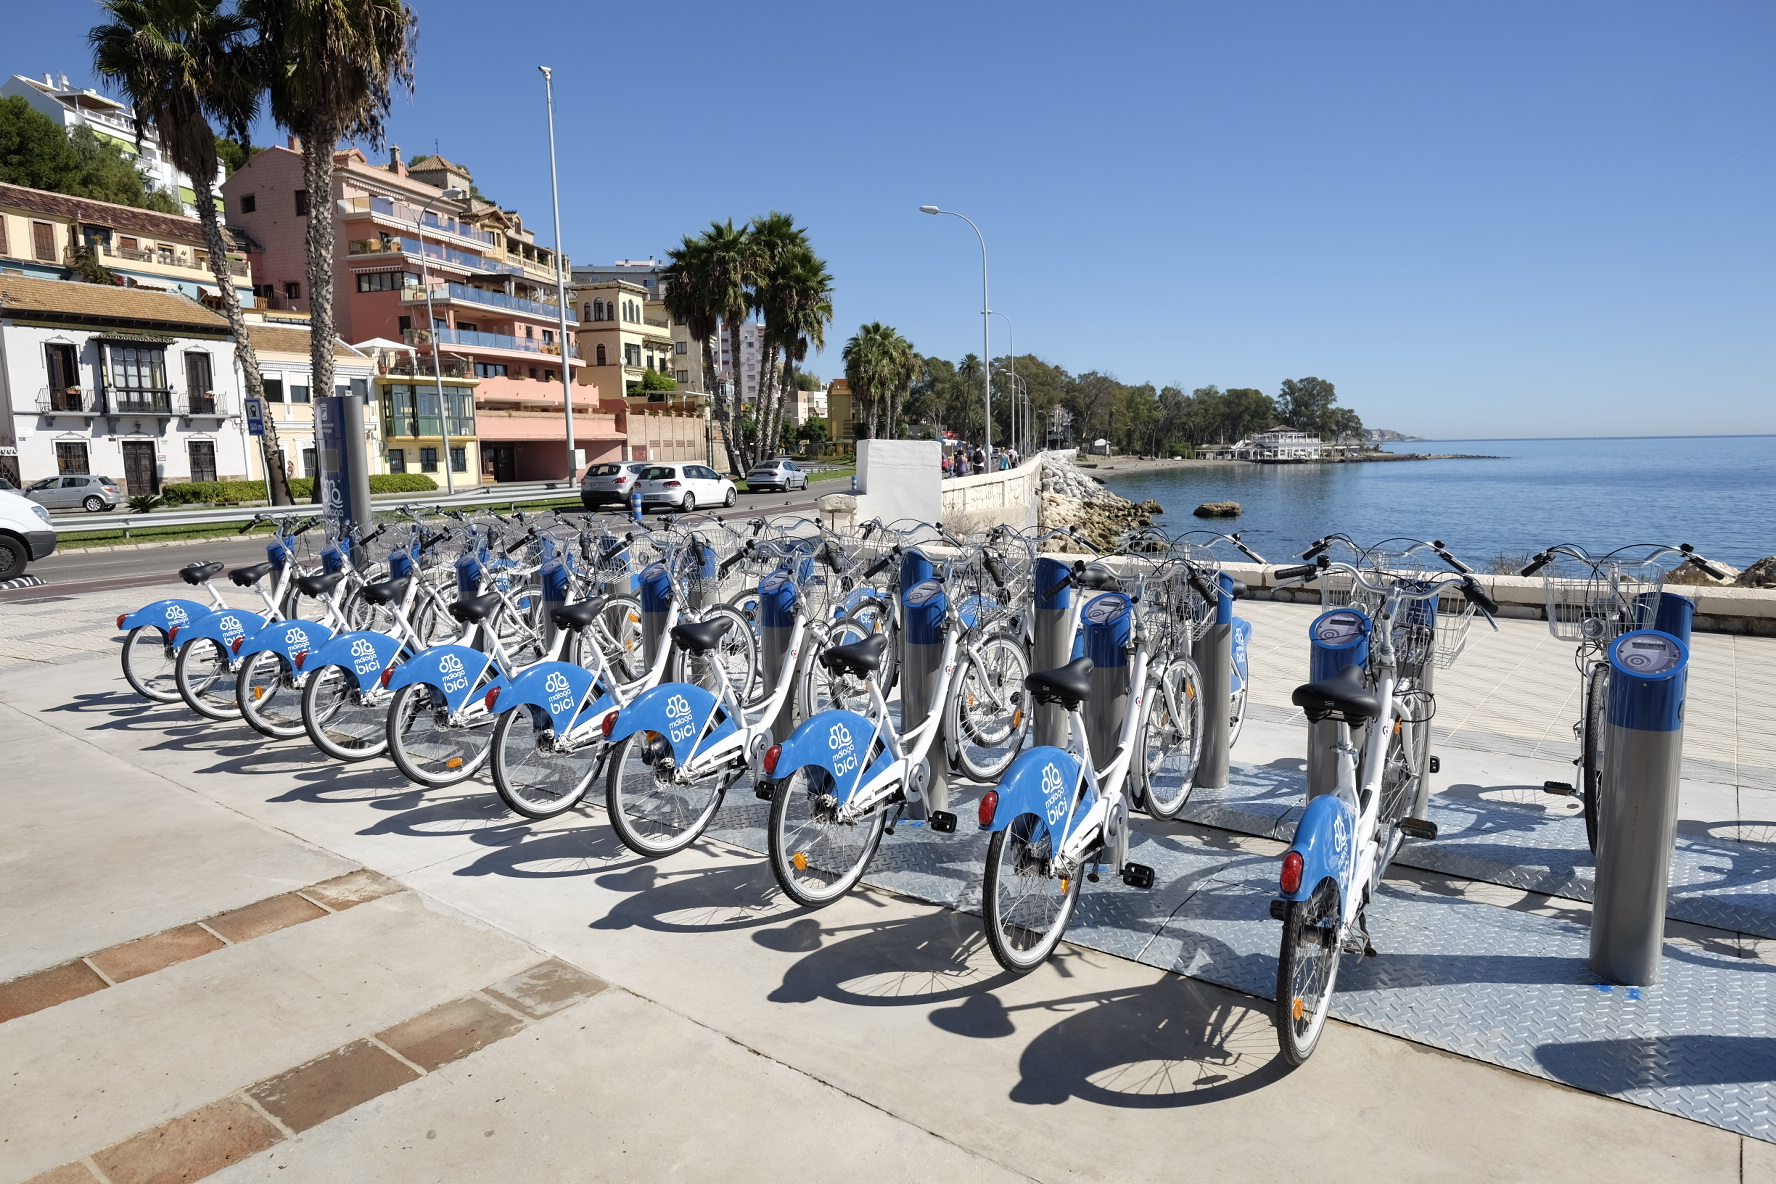
\includegraphics[width=0.8\textwidth]{graphs/bici-por-malaga}
	\caption{Aparcamiento de bicicletas p�blicas de la ciudad de M�laga}
	\label{fig:bici-por-malaga}
\end{figure}

La idea de funcionamiento ser�a simple el usuario llegar�a a las bicicletas, y le llegar�a una notificaci�n de la web f�sica con un enlace donde poder elegir una bicicleta y al seleccionar una, el candado de esta se abrir�a. De este funcionamiento en este proyecto solamente se ha abordado la parte de poder enviar la informaci�n desde la web al nodo, dejando lo dem�s como l�nea futura de este \ac{TFG}.


\chapterend{}

\chapterbegin{Descripci�n general del proyecto}
\label{chp:ti15stack}
\minitoc
\begin{figure}[h]
	\centering
	\def\svgwidth{\columnwidth}
	\resizebox{\textwidth}{!}{\input{graphs/diagramaGeneral.pdf_tex}}
	\caption{Esquema general del proyecto}
\end{figure}

\sectionx{Visi�n General}
Probando t�ldes
\sectionx{Ti 15.4 Stack}

\sectionx{Raspberry Pi}

\sectionx{Protocol Buffers}

\sectionx{NodeJS}


\chapterend
%\chapterbegin{Estructura del documento}
\label{chp:estructura}
%\minitoc




\chapterend{}
%\chapterbegin{Especificaciones}
\label{chp:especificaciones}
\minitoc

\sectionx{Especificaciones principales}

\sectionx{Especificaciones secundarias}

\chapterend{}
\chapterbegin{Estado del arte}
\label{chp:estadoArte}
\minitoc

\sectionx{Web f\'{i}sica}
	\begin{wrapfigure}{r}{0.4\textwidth}
	\begin{center}
		
\includegraphics[width=0.2\textwidth]{graphs/phyWeb-logo}
	\end{center}
	\caption{Logo de la web f\'{i}sica}
\end{wrapfigure}

El primer concepto que hay que conocer para afrontar el proyecto es el de Web F�sica. La Web F�sica es un t�rmino que describe el proceso de presentar objetos cotidianos en internet\cite{enablingInternetThings}. Este enfoque ofrece a los usuarios m�viles la posibilidad de gestionar sus tareas diarias en el uso de objetos cotidianos. Los objetos comienzan a ser inteligentes y remotamente controlables. Este modelo permite a los usuarios m�viles navegar y controlar los objetos f�sicos que rodean al dispositivo m�vil. Adem�s, esto ayuda al desempe�o de tareas diarias dependiendo de los objetos cercanos \cite{phisicalWebSmartCities}.\\

Podemos mencionar en este contexto a los conocidos c�digos \ac{QR}, los c�digos \ac{QR} son un c�digo de barras en dos dimensiones, a menudo utilizados para mapear \ac{URL} con objetos f�sicos \cite{recognitionQRCodeMobile}.\\

Las etiquetas inal�mbricas son uno de los enfoques m�s utilizados para el marcado de objetos f�sicos. Las etiquetas inal�mbricas pueden soportar protocolos como \ac{BLE} y \textit{WiFi}. Los protocolos mencionados son soportados por la mayor�a de los tel�fonos m�viles modernos.\\


\begin{figure}[h]
	\centering
	\def\svgwidth{\columnwidth}
	\resizebox{0.7\textwidth}{!}{\input{graphs/dibujo.pdf_tex}}
	\caption{Ejemplos de comunicaci\'{o}n cercana}
\end{figure}

En la Web F�sica, personas, lugares y objetos tienen p�ginas web que proveen informaci�n y mecanismos de interacci�n. Sin embargo, es la amplitud y la profundidad de la pila que rodea a la web, que hacen de esta una atractiva visi�n para la evoluci�n del \ac{IOT}.\cite{enablingInternetThings}\\

Las p�ginas web son una fant�stica tecnolog�a para interacci�n \ac{H2M}, pero muchos de los casos de uso del \ac{IOT} son interacciones \ac{M2M}. Los formatos de datos usados por \url{Schema.org} y otros, permiten a los agentes de usuario y servicios en la nube analizar los datos para eventos, organizaciones, personas, lugares, productos y as� sucesivamente, acutando sobre ellos de forma interactiva y proactiva.  \cite{enablingInternetThings}\\

Uno de los primeros proyectos en fomentar esta idea fue \ac{HP} con \textit{Cooltown}, que usaba balizas infrarrojas para transmitir URLs. M�s recientemente, \ac{BLE} proporciona una similar baliza de bajo consumo que puede emitir \ac{URL} en paquetes peri�dicos (\url{www.uribeacon.org}). \cite{enablingInternetThings}\\


\sectionx{Redes inal\'{a}mbricas e internet de las cosas}

\subsection*{Introducci�n}
El futuro de internet tiene como meta integrar diferentes tecnolog�as de comunicaci�n, cableadas e inal�mbricas, con el objetivo de contribuir sustancialmente a mejorar el concepto de \ac{IOT} \cite{smartObjectBlock}. Aunque hay muchas maneras de describir el \ac{IOT}, podemos definirlo como una red con objetos interconectados con direcciones �nicas, basadas en un protocolo est�ndar de comunicaci�n.\cite{evolutionWirelesSensorNetworks}\\

Los sensores de bajo costo han facilitado la proliferaci�n de \ac{WSN} en muchos escenarios como monitorizaci�n medioambiental, agricultura, salud, y construcciones inteligentes. \ac{WSN} est�n caracterizadas por una alta heterogeneidad porque est�n basadas en diferentes soluciones, propietarias y no propietarias. Este gran rango de soluciones est� retrasando actualmente desarrollos a gran escala de estas tecnolog�as a fin de que se obtenga una gran red virtual de sensores que permita integrar todos las existentes redes de sensores.\cite{fromTodayFutureInternet}\\

Las redes de sensores basadas en sistemas cerrados o propietarios son islas conectivamente hablando, con limitadas comunicaciones con el mundo exterior. Por lo general, es necesario usar \textit{gateways} con conocimiento espec�fico de la aplicaci�n para exportar los datos de la \ac{WSN} a otros dispositivos conectados a Internet. Adem�s, no hay comuniaci�n directa entre diferentes protocolos a menos que se implementen complejas conversiones espec�ficas para la aplicaci�n en los \textit{gateways} o \textit{proxies}.

\subsection*{Visi\'{o}n general de las soluciones existentes}
En este apartado presentaremos una r�pida visi�n general de las principales tecnolog�as usadas para \ac{WSN} \cite{wirelessAutomationNetworks}. Analizaremos las soluciones que no est�n basadas en los protocolos de internet. 

\subsubsection*{ZIGBEE} 
ZigBee es una tecnolog�a de red inal�mbrica desarrollada por la ZigBee Alliance para baja tasa de transmisi�n de datos y aplicaciones de corto alcance \cite{ZigBeeHome}. La pila de protocolos ZigBee  est� compuesta por 4 principales capas: la capa \ac{PHY}, la capa \ac{MAC}, la capa \ac{NWK} y la capa \ac{APL}. \ac{PHY} y \ac{MAC} de ZigBee est�n definidas por el est�ndar \ac{IEEE} 802.15.4, mientras el resto de la pila est� definida por la especificaci�n ZigBee.\\

Esta versi�n inicial del \ac{IEEE} 802.15.4, en la que ZigBee est� basado, funciona en la bandas de 868 MHz (Europa), 915 MHz (Norteam�rica) y 2.4 GHz (global).\\

Una nueva especificaci�n de ZigBee es RF4CE \cite{ZigBeeRF4C}, que tiene una simplificada pila de red para topolog�as en estrellas solamente, ofreciendo una soluci�n simple para el control remoto de electr�nica de consumo.

\subsubsection*{Z-WAVE} Z-Wave es un protocolo inal�mbrico desarrollado por ZenSys y promovida por la Z-Wave Alliance para automatizaciones residenciales y peque�os entornos comerciales. El principal objetivo de permitir transmisiones seguras de cortos mensajes desde una unidad de control hasta uno m�s nodos en la red \cite{ZWaveProtocol}. Z-Wave esta organizado de acuerdo a un arquitectura cumpuesta por 5 capas principales: \ac{PHY}, \ac{MAC}, transferencia, enrutado y capas de aplicaci�n.\\

Z-Wave opera principalmente en la banda de 900 MHz (868 MHz en Europa y 908 MHz en Estados Unidos) y 2.4 GHz. Z-Wave permite tasas de transmisi�n a 9.6 kb/s, 40 kb/s y 200 kb/s.

\subsubsection*{INSTEON}
INSTEON \cite{InsteonDetails} es una soluci�n desarrollada por SmartLabs y promovida por la INSTEON Alliance. Una de las distintivas caracter�sticas de INSTEON es el hecho de como define una topolog�a de red compuesta de \ac{RF} y \textit{power line links}. Los dispositivos pueden ser \ac{RF},  \textit{power-line}, o pueden soportar ambos tipos de comunicaci�n.\\

INSTEON opera a 904 MHz como frecuencia central, con una tasa de datos bruta de 38.4 kb/s.\\

Los dispositivos INSTEON son duales, lo que significa que cualquiera de ellos pueden tener el rol de emisor, receptor o repetidor. La comunicaci�n entre ambos dispositivos que no est�n en el mismo rango se logra mediante un enfoque <<multisalto>> que usa los repetidores en un esquema de sincronizaci�n temporal.

\subsubsection*{WAVENIS}
Wavenis es un protocolo inal�mbrico desarrollado por Coronis System para el control y monitorizaci�n de aplicaciones en entornos exigentes, incluida la dom�tica y la automatizaci�n de edificios. Wavenis actualmente est� promovida y gestionada por la \ac{Wavenis-OSA}. Est� definido por la funcionalidad de las capas f�sica, de enlace y de red \cite{ProblemSolvingWireless}. Los servicios de Wavenis pueden ser accedidos desde capas superiores mediante una \ac{API}.\\

Wavenis opera principalmente en las bandas de 433 MHz, 868 MHz y 915 MHz, que son bandas reservadas para \ac{ISM} en Asia, Europa y Estados Unidos. Algunos productos tambi�n operan en la banda de 2.4 GHz. Las tasas de transmisi�n m�nimas y m�ximas dadas por Wavenis son 4.8 kb/s y 100 kb/s, respectivamente, con 19.2 kb/s como valor t�pico.

\subsubsection*{IEEE 802.15.4}

% TODO REVISAR ESTE APARTADO
El est�ndar del IEEE 802.15.4, define las especificaciones de la capa f�sica y la subcapa de acceso al medio para conectividad inal�mbrica con baja tasa de datos y bajo consumo de energ�a. Una red 802.15.4 puede simplemente funcionar como una red en estrella con un �nico salto o, cuando las distancias son grandes, puede funcionar como una red en estrella multisalto. \cite{zheng2006comprehensive}\\

Los enlaces inal�mbricos utilizando 802.15.4 pueden operar en tres bandas \ac{ISM}. En total 27 canales son utilizables en 802.15.4, donde 16 canales en la banda de 2.4GHz, 10 canales en la banda de 915MHz y 1 canal en la banda de 868MHz.



\chapterend{}

%
\chapterbegin{Metodolog�a y directrices seguidas}
\label{chp:metod}



\chapterend
%\chapterbegin{Web f\'{i}sica}
\label{chp:webfisica}
\minitoc
	
	\begin{wrapfigure}{r}{0.4\textwidth}
		\begin{center}
			
\includegraphics[width=0.2\textwidth]{graphs/phyWeb-logo}
		\end{center}
		\caption{Logo de la web f\'{i}sica}
	\end{wrapfigure}
	
	El primer concepto que hay que conocer para afrontar el proyecto es el de Web F�sica. La Web F�sica es un t�rmino que describe el proceso de presentar objetos cotidianos en internet\cite{enablingInternetThings}. Este enfoque ofrece a los usuarios m�viles la posibilidad de gestionar sus tareas diarias en el uso de objetos cotidianos. Los objetos comienzan a ser inteligentes y remotamente controlables. Este modelo permite a los usuarios m�viles navegar y controlar los objetos f�sicos que rodean al dispositivo m�vil. Adem�s, esto ayuda al desempe�o de tareas diarias dependiendo de los objetos cercanos \cite{phisicalWebSmartCities}.\\
	
	Podemos mencionar en este contexto a los conocidos c�digos \ac{QR}, los c�digos \ac{QR} son un c�digo de barras en dos dimensiones, a menudo utilizados para mapear \ac{URL} con objetos f�sicos \cite{recognitionQRCodeMobile}.\\
	
	Las etiquetas inal�mbricas son uno de los enfoques m�s utilizados para el marcado de objetos f�sicos. Las etiquetas inal�mbricas pueden soportar protocolos como \ac{BLE} y \textit{WiFi}. Los protocolos mencionados son soportados por la mayor�a de los tel�fonos m�viles modernos.\\
	
	
	\begin{figure}
		\centering
		\def\svgwidth{\columnwidth}
		\resizebox{0.7\textwidth}{!}{\input{graphs/dibujo.pdf_tex}}
		\caption{Ejemplos de comunicaci\'{o}n cercana}
	\end{figure}
	
	En la Web F�sica, personas, lugares y objetos tienen p�ginas web que proveen informaci�n y mecanismos de interacci�n. Sin embargo, es la amplitud y la profundidad de la pila que rodea a la web, que hacen de esta una atractiva visi�n para la evoluci�n del \ac{IOT}.\cite{enablingInternetThings}\\
	
	Las p�ginas web son una fant�stica tecnolog�a para interacci�n \ac{H2M}, pero muchos de los casos de uso del \ac{IOT} son interacciones \ac{M2M}. Los formatos de datos usados por \url{Schema.org} y otros, permiten a los agentes de usuario y servicios en la nube analizar los datos para eventos, organizaciones, personas, lugares, productos y as� sucesivamente, acutando sobre ellos de forma interactiva y proactiva.  \cite{enablingInternetThings}\\
	
	Uno de los primeros proyectos en fomentar esta idea fue \ac{HP} con \textit{Cooltown}, que usaba balizas infrarrojas para transmitir URLs. M�s recientemente, \ac{BLE} proporciona una similar baliza de bajo consumo que puede emitir \ac{URL} en paquetes peri�dicos (\url{www.uribeacon.org}). \cite{enablingInternetThings}\\
	
	
\chapterend{}
%\chapterbegin{Redes inal\'{a}mbricas e internet de las cosas}
\label{chp:redes}
\minitoc


El futuro de internet tiene como meta integrar diferentes tecnolog�as de comunicaci�n, cableadas e inal�mbricas, con el objetivo de contribuir sustancialmente a mejorar el concepto de \ac{IOT} \cite{smartObjectBlock}. Aunque hay muchas maneras de describir el \ac{IOT}, podemos definirlo como una red con objetos interconectados con direcciones �nicas, basadas en un protocolo est�ndar de comunicaci�n.\cite{evolutionWirelesSensorNetworks}\\

Los sensores de bajo costo han facilitado la proliferaci�n de \ac{WSN} en muchos escenarios como monitorizaci�n medioambiental, agricultura, salud, y construcciones inteligentes. \ac{WSN} est�n caracterizadas por una alta heterogeneidad porque est�n basadas en diferentes soluciones, propietarias y no propietarias. Este gran rango de soluciones est� retrasando actualmente desarrollos a gran escala de estas tecnolog�as a fin de que se obtenga una gran red virtual de sensores que permita integrar todos las existentes redes de sensores.\cite{fromTodayFutureInternet}\\

%TODO a�adir imagen  "Interworking among heterogeneous WSNs. " de la cita: fromTodayFutureInternet
Las redes de sensores basadas en sistemas cerrados o propietarios son islas conectivamente hablando, con limitadas comunicaciones con el mundo exterior. Por lo general, es necesario usar \textit{gateways} con conocimiento espec�fico de la aplicaci�n para exportar los datos de la \ac{WSN} a otros dispositivos conectados a Internet. Adem�s, no hay comuniaci�n directa entre diferentes protocolos a menos que se implementen complejas conversiones espec�ficas para la aplicaci�n en los \textit{gateways} o \textit{proxies}.

\sectionx{Visi\'{o}n general de las soluciones existentes}
En este apartado presentaremos una r�pida visi�n general de las principales tecnolog�as usadas para \ac{WSN} \cite{wirelessAutomationNetworks}. Analizaremos las soluciones que no est�n basadas en los protocolos de internet. 

\subsection*{ZIGBEE} 
ZigBee es una tecnolog�a de red inal�mbrica desarrollada por la ZigBee Alliance para baja tasa de transmisi�n de datos y aplicaciones de corto alcance \cite{ZigBeeHome}. La pila de protocolos ZigBee  est� compuesta por 4 principales capas: la capa \ac{PHY}, la capa \ac{MAC}, la capa \ac{NWK} y la capa \ac{APL}. \ac{PHY} y \ac{MAC} de ZigBee est�n definidas por el est�ndar \ac{IEEE} 802.15.4, mientras el resto de la pila est� definida por la especificaci�n ZigBee.\\

Esta versi�n inicial del \ac{IEEE} 802.15.4, en la que ZigBee est� basado, funciona en la bandas de 868 MHz (Europa), 915 MHz (Norteam�rica) y 2.4 GHz (global).\\

Una nueva especificaci�n de ZigBee es RF4CE \cite{ZigBeeRF4C}, que tiene una simplificada pila de red para topolog�as en estrellas solamente, ofreciendo una soluci�n simple para el control remoto de electr�nica de consumo.

\subsection*{Z-WAVE} Z-Wave es un protocolo inal�mbrico desarrollado por ZenSys y promovida por la Z-Wave Alliance para automatizaciones residenciales y peque�os entornos comerciales. El principal objetivo de permitir transmisiones seguras de cortos mensajes desde una unidad de control hasta uno m�s nodos en la red \cite{ZWaveProtocol}. Z-Wave esta organizado de acuerdo a un arquitectura cumpuesta por 5 capas principales: \ac{PHY}, \ac{MAC}, transferencia, enrutado y capas de aplicaci�n.\\

Z-Wave opera principalmente en la banda de 900 MHz (868 MHz en Europa y 908 MHz en Estados Unidos) y 2.4 GHz. Z-Wave permite tasas de transmisi�n a 9.6 kb/s, 40 kb/s y 200 kb/s.

\subsection*{INSTEON}
INSTEON \cite{InsteonDetails} es una soluci�n desarrollada por SmartLabs y promovida por la INSTEON Alliance. Una de las distintivas caracter�sticas de INSTEON es el hecho de como define una topolog�a de red compuesta de \ac{RF} y \textit{power line links}. Los dispositivos pueden ser \ac{RF},  \textit{power-line}, o pueden soportar ambos tipos de comunicaci�n.\\

INSTEON opera a 904 MHz como frecuencia central, con una tasa de datos bruta de 38.4 kb/s.\\

Los dispositivos INSTEON son parejas, lo que significa que cualquiera de ellos pueden tener el rol de emisor, receptor o repetidor. La comunicaci�n entre ambos dispositivos que no est�n en el mismo rango se logra mediante un enfoque <<multisalto>> que usa los repetidores en un esquema de sincronizaci�n temporal.

\subsection*{WAVENIS}
Wavenis es un protocolo inal�mbrico desarrollado por Coronis System para el control y monitorizaci�n de aplicaciones en entornos exigentes, incluida la dom�tica y la automatizaci�n de edificios. Wavenis actualmente est� promovida y gestionada por la \ac{Wavenis-OSA}. Est� definido por la funcionalidad de las capas f�sica, de enlace y de red \cite{ProblemSolvingWireless}. Los servicios de Wavenis pueden ser accedidos desde capas superiores mediante una \ac{API}.\\

Wavenis opera principalmente en las bandas de 433 MHz, 868 MHz y 915 MHz, que son bandas reservadas para \ac{ISM} en Asia, Europa y Estados Unidos. Algunos productos tambi�n operan en la banda de 2.4 GHz. Las tasas de transmisi�n m�nimas y m�ximas dadas por Wavenis son 4.8 kb/s y 100 kb/s, respectivamente, con 19.2 kb/s como valor t�pico.

\subsection*{TI 15.4-STACK}
El TI 15.4-Stack es una plataforma completa libre de derechos de autor para desarrollar aplicaciones que requieren una soluci�n inal�mbrica con topolog�a en estrella, un extremado bajo consumo, largo alcance, fiable, robusto y seguro.\\

Este cap�tulo \ref{chp:ti154} se explicar� en detalle las caracter�sticas de este protocolo y el uso en este proyecto.

\chapterend{}
%\chapterbegin{Plataformas para comunicaciones inal�mbricas}
\label{chp:plataformasComunicaciones}
\minitoc

\sectionx{ESP8266}

\sectionx{Intel Edison}



\chapterend{}
%\chapterbegin{Plataformas basadas en Linux}
\label{chp:plataformasLinux}
\minitoc

\sectionx{BeagleBone Black}

\sectionx{Raspberry Pi}


\chapterend{}

\part{Desarrollo del proyecto}


\chapterbegin{Red inal�mbrica}
\label{chp:redInalambrica}
\minitoc

\section{Introducci�n}

La red inal�mbrica es la parte de este \ac{TFG} que engloba al nodo y al concentrador (v�ase figura \ref{fig:esquemaGeneral}). En este cap�tulo se detallan las caracter�sticas y funcionamiento de cada de las partes.

\section{Nodo}



\subsection*{Introducci�n}

La aplicaci�n implementa el dispositivo de la red, que le permite conectarse a la red creada por el concentrador. El sensor peri�dicamente env�a reportes de datos en intervalos configurados por el concentrador y este responde con mensajes de rastreo.

\subsection*{Arquitectura Hardware}

\subsection*{ARM Cortex M0 (N�cleo radio)}
El n�cleo \ac{CM0} en el CC1350 es responsable de la interfaz audio, y traduce complejas instrucciones del n�cleo \ac{CM3}  en bits que son enviados a trav�s del enlace radio.  Para el protocolo TI 15.4-Stack, el \ac{CM0} implementa la capa \ac{PHY} de la pila de protocolos. \\

El \textit{firmware} del n�cleo de radio no est� destinado a ser usado o modificado por la aplicaci�n del desarrollador.

\begin{figure}[H]
	\centering
	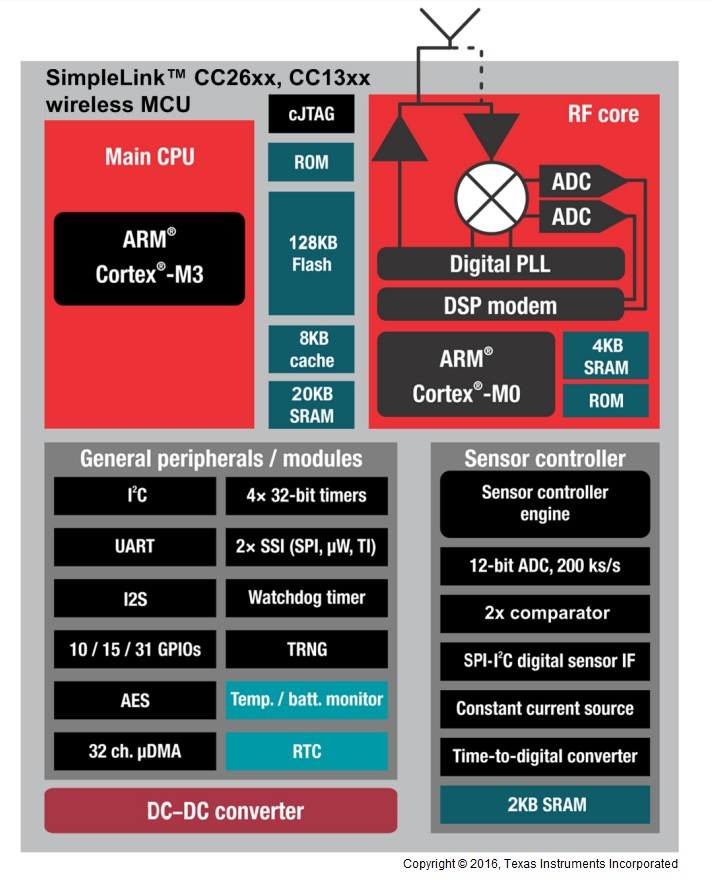
\includegraphics[width=0.5\textwidth]{graphs/fig-simplelink-block-diagram.jpeg}
	\caption{Diagrama de bloques de Simplelink\TM CC13x0}
	\label{fig:diagramaBloquesSimpleLink}
\end{figure}

\subsubsection*{ARM Cortex M3 (N�cleo del sistema)}

El n�cleo \ac{CM3} est� dise�ado para ejecutar la pila del protocolo inal�mbrico desde la capa de enlace hasta la capa de aplicaci�n de usuario. La capa de enlace act�a como interfaz del n�cleo de radio c�mo un m�dulo software llamado \textit{RF driver}.

\subsubsection*{Flash, RAM y perif�ricos}

El CC1350 contiene en el sistema 128KB de memoria flash programable, 20KB de SRAM, y un amplio rango de perif�ricos. La memora flash se divide en partes que se pueden borrar de 4KB. El CC1350 tambi�n contiene 8kB de cach� SRAM que puede ser utilizada para extender la capacidad de la RAM o puede funcionar como una cach� normal para incrementar el rendimiento de la aplicaci�n. Otros perif�ricos incluidos son UART, I2C, I2S, AES, TRNG, temperatura y monitor de la bater�a.



\subsection*{TI-RTOS}

TI-RTOS es un entorno operativo para proyectos TI 15.4-Stack en dispositivos CC1350. El kernel TI-RTOS es una versi�n adaptada del kernel SYS/BIOS y funciona como un sistema operativo con controladores en tiempo real, con prioridades, multitarea y herramientas para la sincronizaci�n y planificaci�n.

% TODO Completar esta secci�n

\subsection*{Arquitectura de la aplicaci�n}

En la figura \ref{fig:fig-example-application-block-diagram} se muestra el diagrama de bloques de la aplicaci�n del nodo.  

\begin{figure}[h]
	\centering
	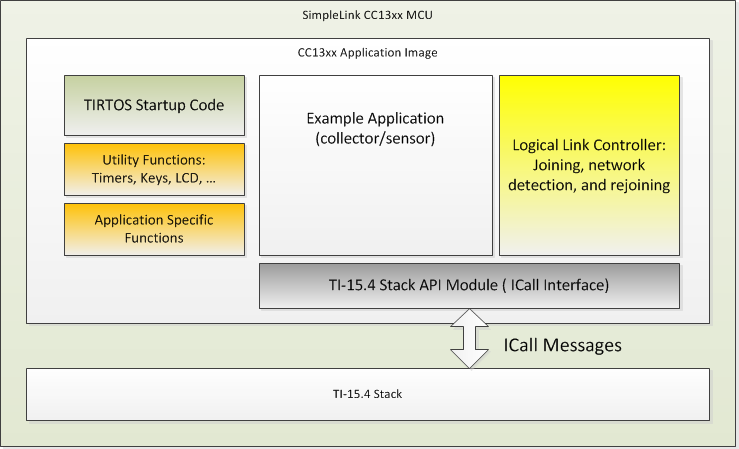
\includegraphics[width=0.8\textwidth]{graphs/fig-example-application-block-diagram}
	\caption{Diagrama de bloques de la aplicaci�n}
	\label{fig:fig-example-application-block-diagram}
\end{figure}


\begin{description}
	\item[Aplicaci�n:] Este bloque contiene la l�gica espec�fica de la aplicaci�n a desarrollar.
	\item[Controlador de l�gica de enlace:] Implementa varias funciones espec�ficas del IEEE 802.15.4 o Wi-SUN (para una configuraci�n \textit{frequency-hopping}) para formaci�n, conexi�n y reconexi�n de la red. 
	\item[Inicio de TI-RTOS:] Inicializa la aplicaci�n.
	\item[Funciones �tiles] Provee varias utilidades para usar LCD, temporizadores, botones y m�s.
	\item[Funciones espec�ficas:] Implementa funciones como guardado de datos, y provee una interfaz para gestionar pulsaciones botones o mostrar informaci�n esencial en un LCD.
	\item[TI 15.4-Stack API (API MAC Module):] Este m�dulo proporciona una interfaz para gesti�n y los servicios de datos del 802.15.4 stack mediante el m�dulo \ac{ICall}.
\end{description}

\subsection*{Funci�n de inicio}

La funci�n \textit{main()} dentro del archivo \textit{main.c} es el punto de inicio de la ejecuci�n de la aplicaci�n. En este punto los componentes relaciones con la placa son inicializados. Las tareas se configuran en eta funci�n, inicializando los par�metros necesarios como su prioridad y su tama�o en la pila. En el paso final, las interrupciones se habilitan y el planificador \textit{SYS/BIOS} se inicia llamando a \textit{BIOS\_start()}.


\subsection*{Arquitectura general de la aplicaci�n}

Esta secci�n describe como la tarea de la aplicaci�n esta estructura en m�s detalle. 

\subsubsection*{Funci�n de inicio de la aplicaci�n}

\begin{wrapfigure}{r}{0.4\textwidth}
	\begin{center}
		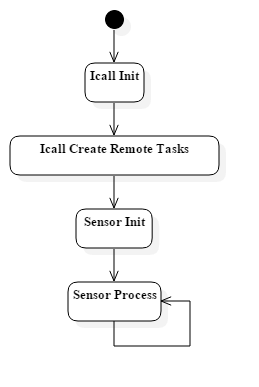
\includegraphics[width=0.4\textwidth]{graphs/TaskFxn.png}
	\end{center}
	\caption{Diagrama de estados de la funci�n de inicio}
\end{wrapfigure}

Despu�s de que la tarea sea construida y el planificador \textit{SYS/BIOS} se inicie, la funci�n que se le pasa durante la construcci�n de la tarea es ejecutada cuando la tarea est� lista.\\

Las funciones de gesti�n de la energ�a son inicializadas aqu� y el m�dulo \ac{ICall} se inicia con la funci�n \textit{ICall\_init()}. La direcci�n IEEE address (programada por TI) es obtenida desde la memoria flash. La tarea de la aplicaci�n (Aplicaci�n Sensor) es inicializada y ejecutada.

\textit{Sensor\_init()} establece varios par�metros de configuraci�n, as� como:

\begin{itemize}
	\item Inicializa las estructuras para los datos
	\item Inicializa el TI 15.4-Stack
	\item Configura la seguridad y el \textit{Logical Link Controller}
	\item Registra las funciones de retorno MAC
\end{itemize} 

\subsection*{Tarea principal}

Despu�s de la funci�n de inicializaci�n, la tarea entra en un bucle infinito ejecutando siempre las mismas tareas,  se puede ver en la figura

\begin{figure}[h]
	\centering
	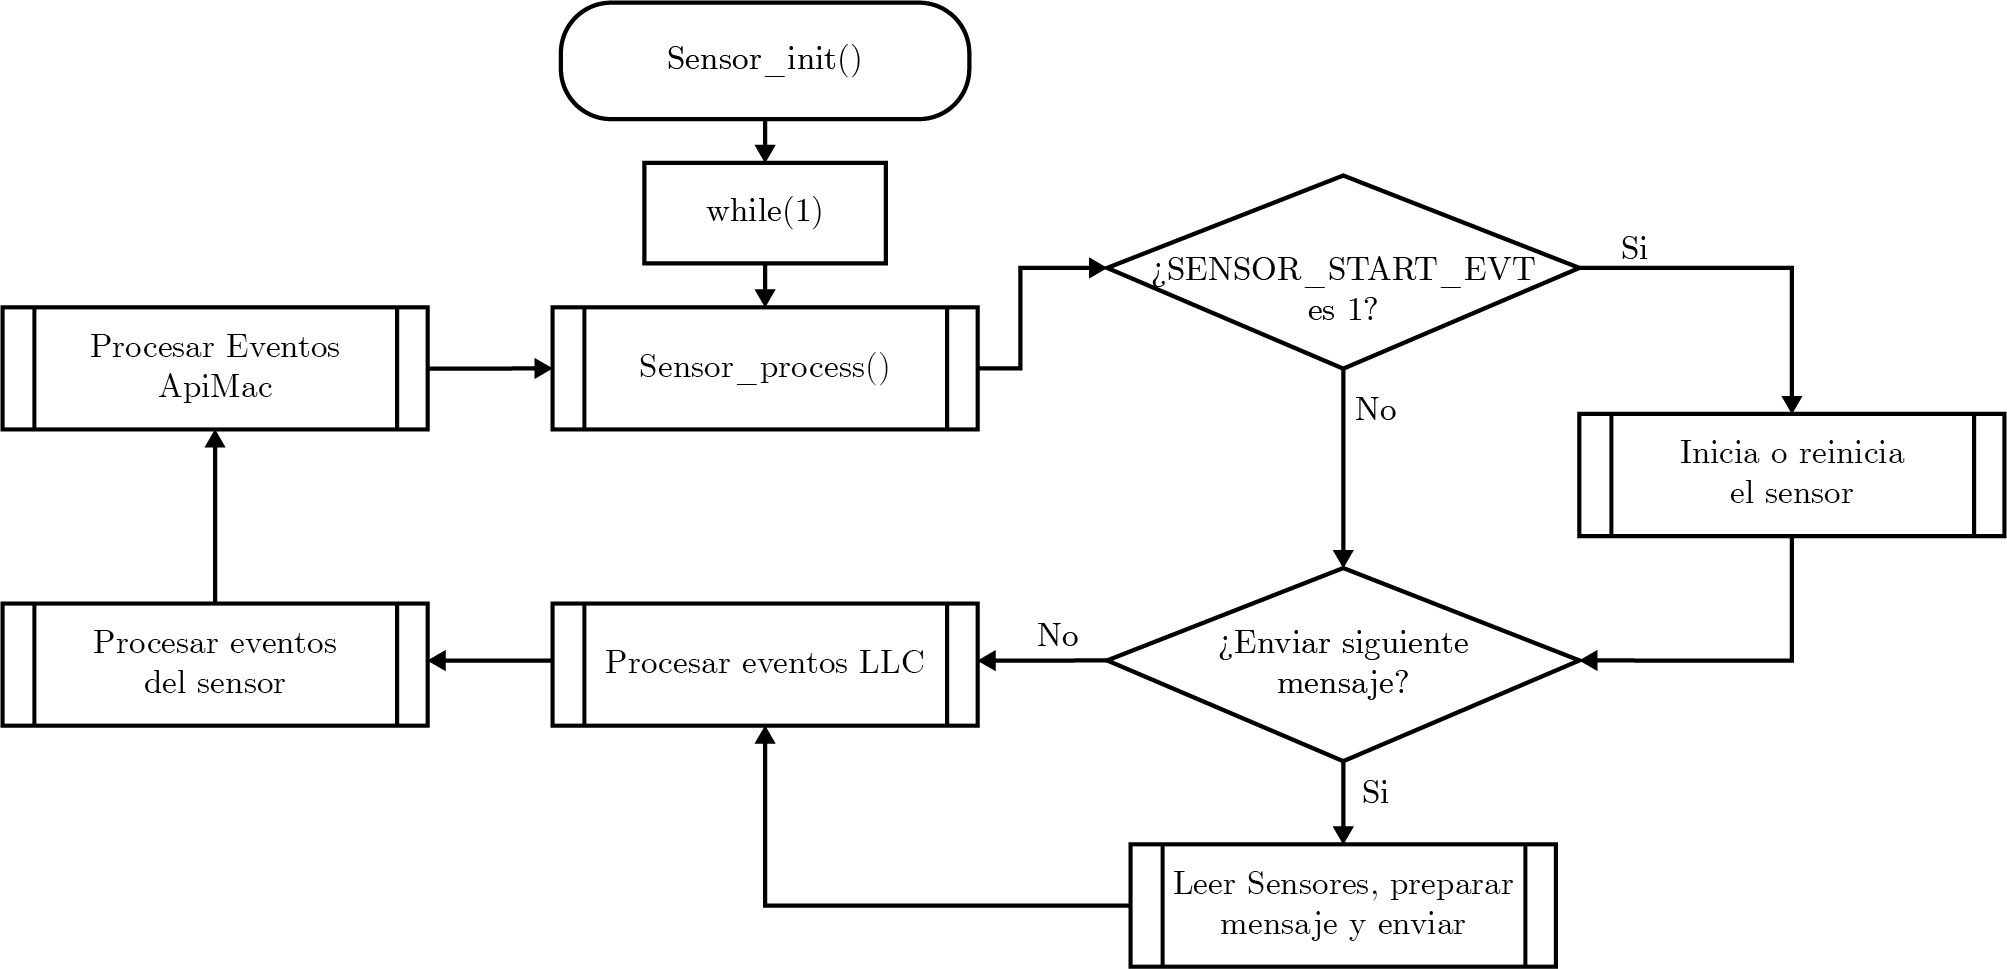
\includegraphics[width=0.8\textwidth]{graphs/fig-sensor-task-flow-chart}
	\caption{Flujo de la aplicaci�n}
	\label{fig:fig-sensor-task-flow-chart}
\end{figure}


\subsection*{Web f�sica}

La librer�a \ac{uBle} permite a la aplicaci�n enviar un paquete en modo \textit{broadcast} a todos los usuarios que est�n en el radio de acci�n del dispositivo. Este paquete de datos es el que utilizamos para notificar a los usuarios con la informaci�n de la web f�sica.\\

Los paquetes bluetooth usan la trama \textit{Eddystone-URL}, estas forman parte del n�cleo de la web f�sica. Una vez el usuario la decodifica la trama podr� acceder a la URL si tiene conexi�n a internet.\\

\subsubsection*{Especificaciones  de la trama}

\begin{table}
	\centering
	\begin{tabular}{|c|c|c|}
		\hline 
		Byte offset & Campo & Descripci�n \\ 
		\hline 
		0 & Tipo de trama & valor = 0x10 \\ 
		\hline 
		1 & Potencia TX & Potencia de TX calibrara a 0 m \\ 
		\hline 
		2 & Prefijo de la URL & Prefijo de la web \\ 
		\hline 
		3+ & URL codificada & Longitud de 1-17 bytes \\ 
		\hline 
	\end{tabular} 
	\caption{Formato de la trama \textit{Eddystone-URL}}
	\label{tab:formatoEddystone}
\end{table}

\begin{description}
	\item[Potencia TX] La potencia de transmisi�n es la potencia recibida a 0 metros, en dBm, en el rango de valores  de -100 dBm a +20dBm con una resoluci�n de 1 dBm.
	\item[Prefijo de la URL] El prefijo de la url define la expansi�n utilizada por la url, por ejemplo ``http://www.'' o ``https://'' son codificadas por los bytes 0x00 o 0x03 respectivamente.
	\item[Sufijo de la URL] El esquema de URL HTTP est� definia por RFC 1738, por ejemplo ``https://goo.gl/S6zT6P'', y es usada para designar recursos accesibles usando HTTP.
\end{description}

\subsection*{Mensajes OTA}

Los posibles mensajes entre el concentrador y el nodo, est�n definidos en el archivo \textit{smsgs.h} (Ap�ndice \ref{apd:estructurasMensajes}) .\\


Ambos, Nodo y Concentrador tienen que tener definidos las mismas estructuras de mensajes para una correcta comunicaci�n.




\section{Concentrador}
\subsection*{Introducci�n}

En este cap�tulo se describe la arquitectura y funcionamiento del concentrador (nodo central). Para este desarrollo se ha utilizado el proyecto de ejemplo que proporciona el fabricante llamado \textit{TI 15.4-Stack Linux Gateway}. \\

La aplicaci�n del concentrador en Linux proporciona la funcionalidad de concentrador de la red, a�adiendo una interfaz como servidor socket para comunicarse con la aplicaci�n \textit{Gateway}. Las aplicaciones del Concentrador y \textit{Gateway} establecen un puente entre el protocolo IEEE 802.15.4 con el protocolo IP siendo una gran punto de comienzo para el \ac{IOT}.

\subsection*{Diagrama de bloques y modelo de la interfaz}
\begin{figure}[h]
	\centering
	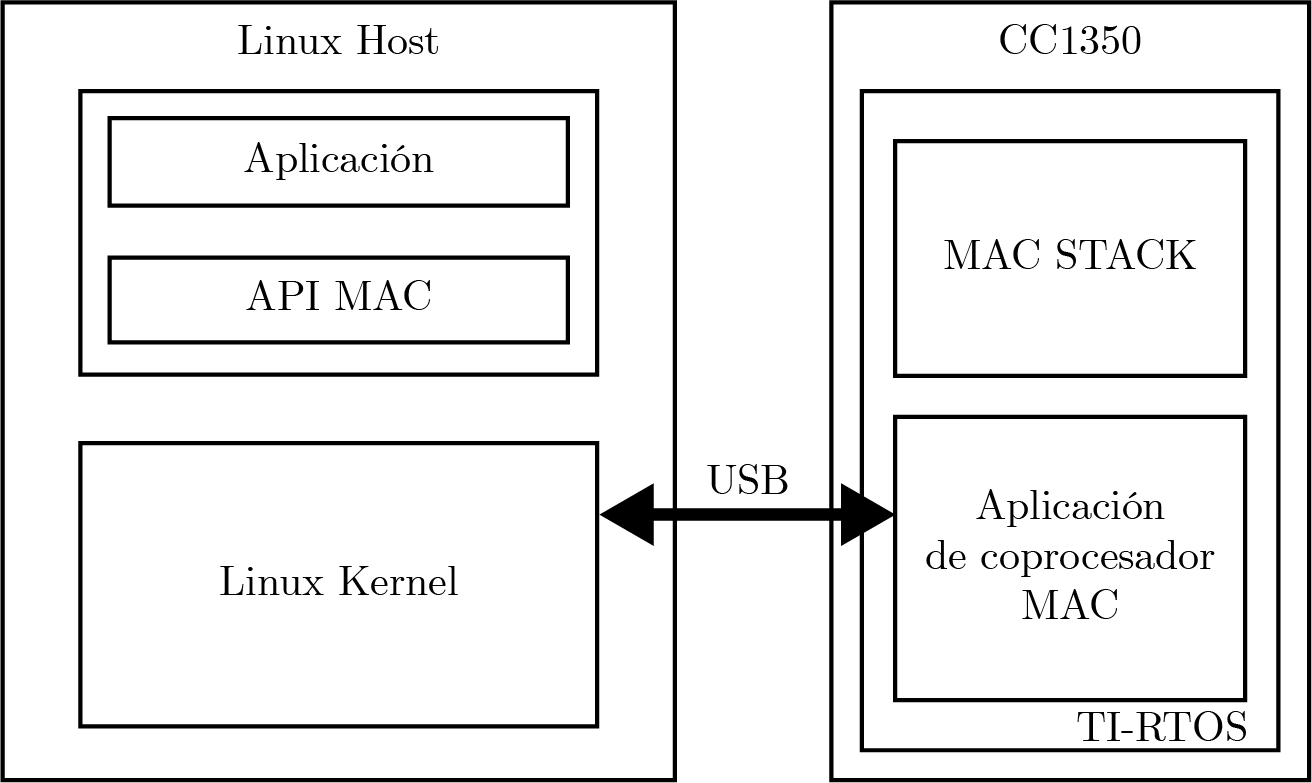
\includegraphics[width=0.8\textwidth]{graphs/concentradorBlockDiagram.png}
	\caption{Arquitectura de software a alto nivel de las aplicaciones TI 15.4-Stack 2.1.0 Linux\R}
	\label{fig:concentradorBlockDiagram}
\end{figure}

Esta secci�n describe la arquitectura de alto nivel basada en coprocesador, los componentes software, y  la arquitectura general del sistema (ve�se figura \ref{fig:concentradorBlockDiagram}). El coprocesador es una entidad que implementa el est�ndar MAC IEEE 802.15.4e/g en un chip dedicado y provee una interfaz serie por la que un procesador externo controla y procesa las operaciones del coprocesador. \\

El concentrador se centra en una arquitectura escalable con una divisi�n perfecta donde el procesador ejecuta las capas sobre el IEEE 802.15.4e/g MAC/PHY.\\

En esta aplicaci�n, el programa se ejecuta en una plataforma basada en Linux. Aunque los componentes de alto nivel , pueden ser conceptualmente aplicados a otras plataformas no basadas en Linux. Los componentes desarrollados ser�n descritos m�s adelante.\\

La interfaz entre el procesador y el coprocesador est�n definidas como capas l�gicas que est�n separadas en esta arquitectura: una capa f�sica (por ejemplo, USB o UART), una capa l�gica de enlace, y la capa de presentaci�n.\\

Componentes software:

\begin{description}
	\item[Aplicaci�n del coprocesador: ] Es el programa ejecutandose en el dispositivo CC1350. Esta aplicaci�n implementa una capa 802.15.4e/g MAC/PHY y proporciona una comunicaci�n serie.
	\item[Kernel Linux]: El kernel Linux provee los controladores para la interfaz serie que est� disponible en un puerto f�sico (por ejemplo, USB).
	\item[Aplicaci�n TI 15.4-Stack: ] Este m�dulo implementa la aplicaci�n usando el protocolo 802.15.4e/g y la estructura del modelo \ac{MT}.
\end{description}

\subsection*{Descripci�n del SDK}
\begin{figure}[h]
	\begin{center}
		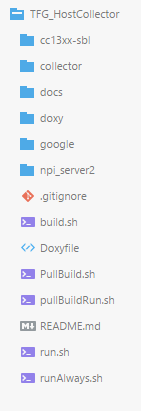
\includegraphics[width=0.5\textwidth]{graphs/fig-oob-dir}
	\end{center}
	\caption{Estructura del directorio TI 15.4-Stack 2.1.0 Linux\R }
	\label{fig:fig-oob-dir}
\end{figure}

La figura \ref{fig:fig-oob-dir} muestra la estructura del directorio de instalaci�n del TI 15.4-Stack 2.1.0. A continuaci�n se explica una descripci�n de alto nivel de cada carpeta:

\begin{description}
	\item[components: ] Contiene las siguientes librer�as:
	\begin{description}
		\item[common: ] Rutinas para caracter�sticas del sistema operativo, como lectura y escritura de ficheros.
		\item[nv: ]  Simula una memoria no vol�til, como la usada en sistemas empotrados.
		\item[api: ] Interfaz de mensajes API MAC y MT
	\end{description}
	\item[docs: ] Documentos como la gu�a de desarrollo y la gu�a de comandos MAC para el coprocesador.
	\item[example: ] Aplicaci�n de ejemplo
	\begin{description}
		\item[cc13xx-sbl: ] Herramientas para la actualizaci�n para los dispositivos CC13x0.
		\item[collector: ]  Aplicaci�n de ejemplo que demuestra como iniciar una red, permitir la conexi�n de dispositivos y recoger datos desde dispositivos remotos.
		\item[gateway: ] Una aplicaci�n basada en Node.js\TM que crea un servidor local y muestra la informaci�n de la red y los datos de los nodos.
		\item[npi\_server2: ] Interfaz socket para comunicarse con el coprocesador.
		\item[google: ] Contiene un makefile para descargar e instalar el compilador de \textit{Google protocol buffer}.
	\end{description}
	\item[firmware] Precompilados ficheros .hex para el coprocesador.
	\item[prebuilt] Compilaci�n para ejecutar la aplicaci�n de ejemplo en una BeagleBone Black.
	\item[scripts] Contiene fragmentos de ficheros makefile usados para compilar la aplicaci�n de ejemplo.
\end{description}

\subsection*{Funcionamiento}

El proyecto comienza en la funci�n \textit{main()}  en el fichero \textit{linux\_main.c}, donde se inicializan las diferentes interfaces, se lee el fichero de configuraci�n y ejecuta la funci�n \textit{App\_main()} del fichero \textit{appsrv.c}.\\

La funci�n \textit{App\_main()} se encarga de inicializar los dos hilos de ejecuci�n principales que tiene el programa, \textit{client-thread} y \textit{collector-thread}. La tarea del cliente se encarga de conectarse al servidor y procesar la transmisi�n y recepci�n de datos por ese canal. Por otro lado la tarea del concentrador, se encarga de generar la red TI 15.4-Stack y procesar los mensajes enviados por este protocolo. \\

\subsubsection*{Hilo del cliente web}
Este hilo mantiene la comunicaci�n con el servidor, y espera recibir un mensaje de este. Cuando un mensaje es recibido la funci�n \textit{appsrv\_handle\_appClient\_request()} es la encargada de procesar el mensaje y notificar a la red TI 15.4-Stack a trav�s del hilo del concentrador.

\subsection*{Hilo del concentrador}

La funci�n \textit{Collector\_process()} del fichero \textit{collector.c} contiene la l�gica de esta tarea, que se describe en la figura ??.

% TODO Incluir figura

\subsection*{Protocol Buffers}

Para facilitar el env�o de datos entre el concentrador y el servidor, se ha utilizado \textit{Protocol Buffers}.\\

\textit{Protocol Buffers} es un mecanismo flexible, eficiente y automatizado para estructurar datos estructurados. Solo es necesario indicar como se estructuran los datos y al compilarse generan la implementaci�n en multiples lenguajes de programaci�n de los mecanismo para codificar y descodificar datos. \\

\subsection*{Funcionamiento}

La estructura de los datos a codificar se definen en archivos .proto. Cada mensaje es una peque�a estructura que contiene una serie de parejas clave-valor. (Ap�ndice \ref{apd:estructurasMensajes} )

Como se observa en el listado \ref{lst:protofield}, el formato de los mensajes es simple y similar a la definici�n de variables en c�digo C. Una vez definidos los mensajes, se ejecuta el compilador de \textit{Protocol Buffers} para el lenguaje de tu aplicaci�n, en nuestro caso C.\\

\lstinputlisting[caption=Ejemplo de estructura con Protocol Buffers,label=lst:protofield,linewidth=\textwidth,breaklines=true,language=C++]{code/Smsgs_msgStatsField.proto}


Las estructuras de datos para nuestra aplicaci�n se pueden observar en el Ap�ndice \ref{apd:estructurasMensajes}. En este podemos observa que hemos creado un fichero con las mismas estructuras a smsgs.h para poder convertir los mensajes que nos llegan de los nodos en mensajes  \textit{Protocol Buffers} y as� poder enviarlos al servidor.





\chapterend{}



\chapterbegin{Servidor}
\label{chp:App}
\minitoc

\section{Introducci�n}


El servidor se puede dividir en dos partes \textit{Front-end} y \textit{Back-End} que son t�rminos que se refieren a la separaci�n entre una capa de presentaci�n y una capa de acceso a datos respectivamente. 

\section{Estructura del directorio}
\begin{figure}[h]
	\centering
	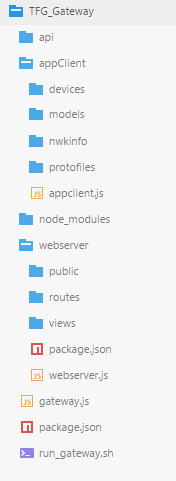
\includegraphics[width=0.2\textwidth]{graphs/estructuraServidor.png}
	\caption{Estructura del directorio del servidor}
	\label{fig:estructuraServidor}
\end{figure}
El servidor est� compuesto por el directorio que se observa en la figura \ref{fig:estructuraServidor} y a continuaci�n se describe la funci�n de cada directorio:

\begin{description}
	\item[api: ] en este directorio se encuentran las definiciones de llamadas \ac{REST} al servidor. Las llamadas \ac{REST} se utilizan para poder acceder a los datos almacenados desde fuera del servidor.
	\item[appClient: ] Esta carpeta contiene el \textit{Back-end} de la web:
	\begin{description}
		\item[devices: ] se definen las funciones relacionadas con la gesti�n de los nodos.
		\item[models: ] aqu� se definen los modelos para guardarlos en la base de datos.
		\item[nwkinfo: ] se definen las funciones relacionadas con la gesti�n del concentrador.
		\item[protofiles: ] aqu� se almacenan los ficheros .proto de \textit{Protocol Buffers}.
		\item[appClient.js: ] en este fichero se inicia el servidor que se comunica con el concentrador y se procesan los mensajes.
	\end{description}
	\item[node\_modules: ] librer�as utilizadas en el proyecto.
	\item[webserver: ] en este directorio est� contenida la l�gica del \textit{Front-end}:
	\begin{description}
		\item[public: ] interfaz del cliente en AngularJS.
		\item[routes: ] Definici�n de rutas.
		\item[views: ] archivos html de las vistas.
		\item[webserver.js: ] se inicia el cliente y se gestiona las peticiones a la web por parte del usuario.
	\end{description}
	\item[gateway.js: ] inicia el \textit{back-end} y el \textit{front-end} y la comunicaci�n entre ambas por \textit{web-sockets}.
	\item[run\_gateway.sh: ] \textit{script} para iniciar el servidor.
\end{description}

\section{Inicio del servidor}

\begin{figure}[H]
	\centering
	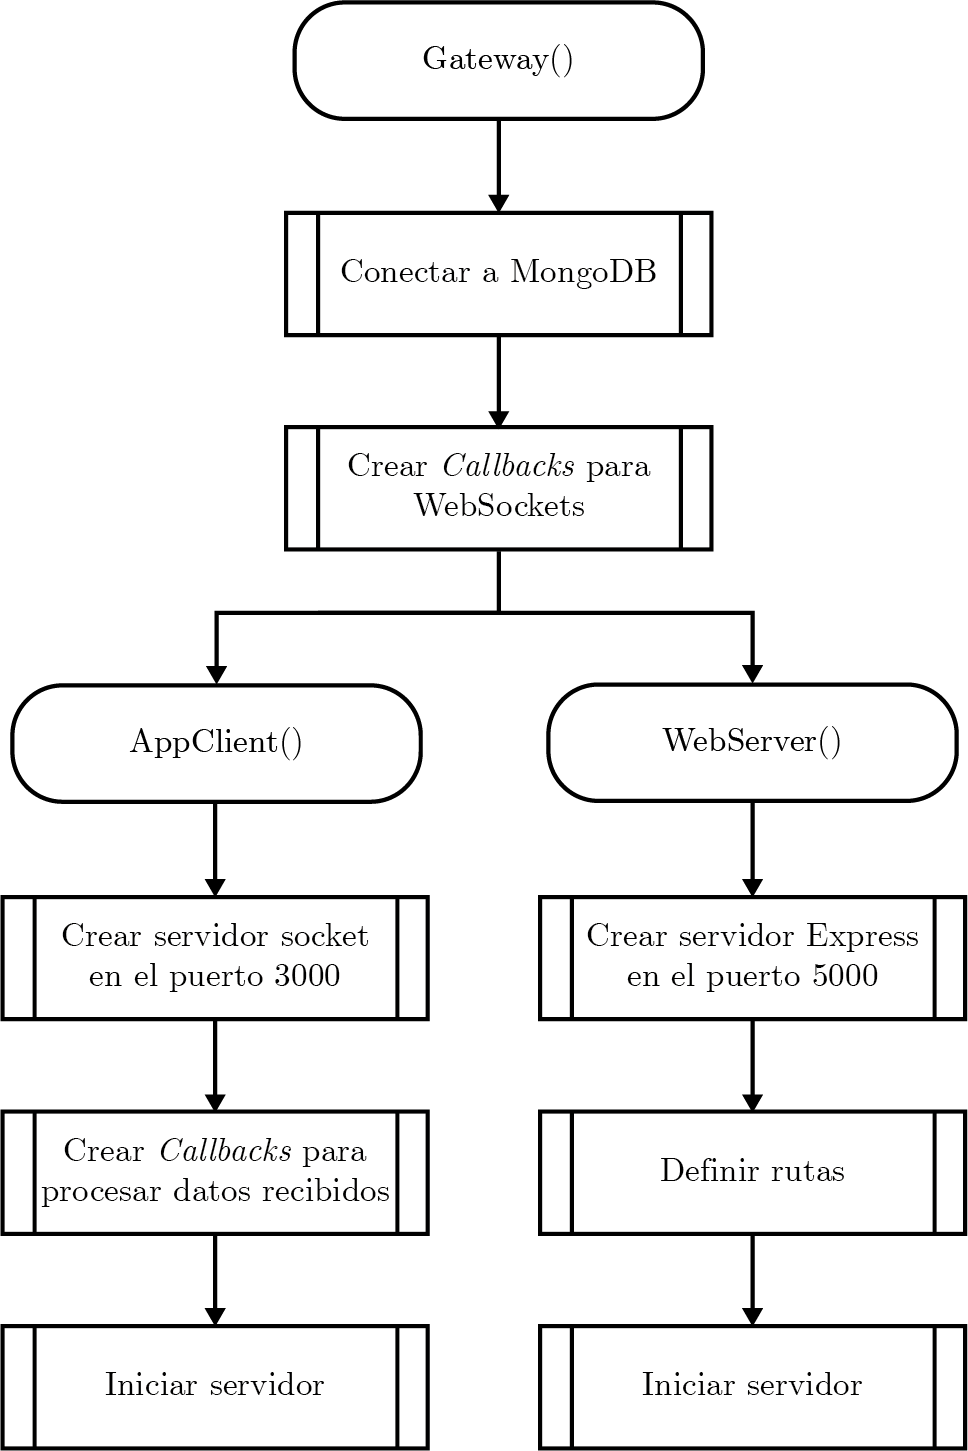
\includegraphics[width=0.6\textwidth]{graphs/fig-server-flow-chart}
	\caption{Diagrama de flujo en el inicio del servidor}
	\label{fig:fig-server-flow-chart}
\end{figure}

La funci�n \textit{Gateway()} inicia todo el servidor, en esta se realiza la conexi�n a la base de datos MongoDB y se crean las funciones \textit{Callbacks} para el intercambio de informaci�n entre el \textit{Back-end} y \textit{Front-end} usando \textit{WebSockets}. La figura \ref{fig:fig-server-flow-chart} refleja el proceso de inicio del servidor.

\section{Back-end}

El \textit{Back-end} es el �rea que se dedica a la l�gica, en este encontramos una interfaz que se encarga de comunicarse con el concentrador y otra que se encarga de comunicarse con el \textit{Front-end} usando \textit{Web-Sockets}.\\

Como se observa en la figura \ref{fig:fig-server-flow-chart}, la funci�n \textit{AppClient()} es la que implementa la creaci�n del servidor en el puerto 3000 para que el concentrador pueda enviar datos al servidor. \\

Cuando la conexi�n entre el concentrador y el collector est� establecida, el \textit{Back-end} queda a la espera de recibir datos del concentrador o del \textit{Front-end}. Todos los datos recibidos del concentrador se almacenan en la base de datos MongoDB para tener un registro de todos los datos de la red que pudieran ser �tiles en un futuro y se env�an al \textit{Front-end}. \\

\subsection{Mensajes enviados entre el concentrador y el Back-end}

En la tabla \ref{tab:appsrv_cmdid} se pueden observar todos los posibles mensajes enviados entre el concentrador y el \textit{Back-end}. Estos mensajes est�n definidos en los ficheros .proto tanto en el concentrador y en el \textit{Back-end}.

\begin{table}[H]
	\centering
	\begin{tabular}{p{0.5\textwidth}|p{0.5\textwidth}}
		\hline 
		\textbf{Identificador de mensaje} &	\textbf{Descripci�n} \\ 
		\hline 
		DEVICE\_JOINED\_IND & Indicaci�n de que un nodo se ha conectado  a la red \\ 
		\hline 
		DEVICE\_LEFT\_IND & Indicaci�n de que un nodo se ha desconectado de la red \\ 
		\hline 
		NWK\_INFO\_IND & Indicaci�n de que est� disponible la informaci�n de la red \\ 
		\hline 
		GET\_NWK\_INFO\_REQ & Petici�n de informaci�n de la red \\ 
		\hline 
		GET\_NWK\_INFO\_RSP & Respuesta de informaci�n de la red \\ 
		\hline 
		GET\_NWK\_INFO\_CNF & Acuse de recibido de GET\_NWK\_ INFO\_RSP \\ 
		\hline 
		GET\_DEVICE\_ARRAY\_REQ & Petici�n de la lista de dispositivos de la red \\ 
		\hline 
		GET\_DEVICE\_ARRAY\_CNF & Acuse de recibido de GET\_DEVICE\_ ARRAY\_REQ \\ 
		\hline 
		DEVICE\_NOTACTIVE\_UPDATE\_IND & Indicaci�n de que un dispositivo no est� activo \\ 
		\hline 
		DEVICE\_DATA\_RX\_IND & Indicaci�n de los datos recibidos de un dispositivo \\ 
		\hline 
		COLLECTOR\_STATE\_CNG\_IND & Indicaci�n del estado del concentrador \\ 
		\hline 
		SET\_JOIN\_PERMIT\_REQ & Petici�n de permiso de conexi�n de nuevos dispositivos \\ 
		\hline 
		SET\_JOIN\_PERMIT\_CNF & Acuse de recibido de SET\_JOIN\_ PERMIT\_REQ \\ 
		\hline 
		TX\_DATA\_REQ & Petici�n de transmisi�n de datos \\ 
		\hline 
		TX\_DATA\_CNF & Acuse de recibido de TX\_DATA\_REQ \\ 
		\hline 
		GET\_COLLECTOR\_STATS\_REQ & Petici�n de las estad�sticas del concentrador \\ 
		\hline 
		GET\_COLLECTOR\_STATS\_RSP & Respuesta con las estad�sticas del concentrador \\ 
		\hline 
	\end{tabular} 
	\caption{Identificadores de los mensajes enviados entre el concentador y el servidor}
	\label{tab:appsrv_cmdid}
\end{table}

\subsection{Mensajes enviados entre el Back-end y Front-end}

Para que se pueda administrar la red y observar todos sus par�metros en el \textit{Front-end} se han creado los mensajes que se observan en la tabla \ref{tab:webSocket} que se env�an a trav�s de \textit{WebSockets}.

\begin{table}[H]
	\centering
	\begin{tabular}{p{0.3\textwidth}|p{0.7\textwidth}}
		\hline 
		\textbf{Identificador} & \textbf{Descripci�n} \\ 
		\hline 
		sendConfig & Env�o de la petici�n de configuraci�n \\ 
		\hline 
		sendToggle & Env�o de conmutaci�n de un led de la placa de un nodo \\ 
		\hline 
		sendToggleBLE & Env�o de conmutaci�n del estado del BLE de  un nodo \\ 
		\hline 
		getDevArrayReq & Obtener la lista de dispositivos \\ 
		\hline 
		getNwkInfoReq & Obtener la informaci�n de la red \\ 
		\hline 
		setJoinPermitReq & Permitir la conexi�n de nuevos dispositivos \\ 
		\hline 
		changeUrl & Cambiar la URL que env�a un nodo \\ 
		\hline 
		bikeSelectReq & Seleccionar una bicicleta en un nodo de tipo aparcamiento \\ 
		\hline 
		collectorStatReq & Obtener las estad�sticas del collector \\ 
		\hline 
		nodeChangePosition & Cambiar las coordenadas de un nodo \\ 
		\hline 
		collChangePosition & Cambiar las coordenadas del concentrador \\ 
		\hline 
		permitJoinCnf & Respuesta del mensaje setJoinPermitReq \\ 
		\hline 
		connDevInfoUpdate & Actualizaci�n de la informaci�n de un nodo \\ 
		\hline 
		nwkUpdate & Actualizaci�n de la informaci�n de la red \\ 
		\hline 
		getdevArrayRsp & Respuesta del mensaje getDevArrayReq \\ 
		\hline 
	\end{tabular} 
	\caption{Tipos de mensajes enviados por WebSocket entre el Back-end y el Front-end}
	\label{tab:webSocket}
\end{table}

\sectionx{Front-end}

El \textit{Front-end} es la interfaz del servidor con el usuario. Para facilitar el control de las vistas se ha utilizado el \textit{framework AngularJS}.\\

Angular es un \textit{framework} \ac{MVC} para la construcci�n de aplicaciones de una �nica p�gina del lado del cliente en HTML y JavaScript.\\
\begin{figure}[H]
	\centering
	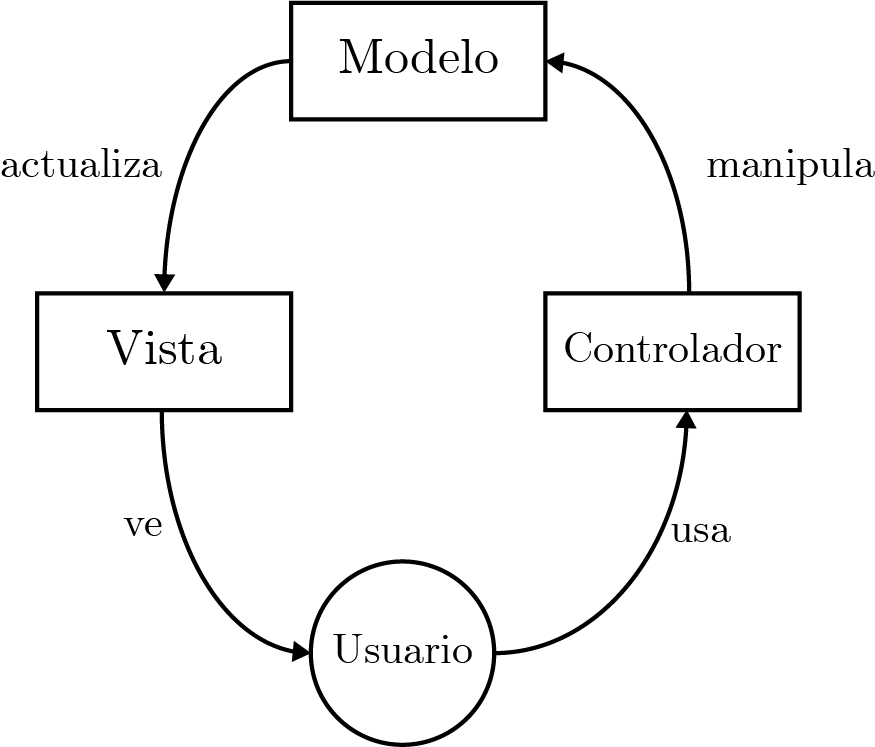
\includegraphics[width=0.6\textwidth]{graphs/fig-mvc}
	\caption{Diagrama de flujo en el inicio del servidor}
	\label{fig:fig-mvc}
\end{figure}
En la figura \ref{fig:fig-mvc} se representa la interacci�n entre las diferentes partes de la arquitectura \ac{MVC}:

\begin{description}
	\item[Vistas: ] Ser� el c�digo HTML y todo lo que presente los datos o informaci�n.
	\item[Controladores: ] Se encarga de toda la l�gica de la aplicaci�n.
	\item[Modelo: ] El modelo es la estructura que define un tipo de dato, y permite acceder a �l en la base de datos.
\end{description}



Todas las funcionalidades del \textit{Front-end} se pueden observar en el manual de uso (Ap�ndice \ref{apd:manual}).


\chapterend{}

\chapterbegin{Pruebas}
\label{chp:pruebas}
\minitoc

\section{Prueba en entorno real}

\subsection{Introducci�n}

Esta prueba consiste en simular el funcionamiento de la red en un entorno lo m�s parecido a un caso de uso real. Para ello se ha instalado el concentrador en un punto fijo como se observa en la figura \ref{fig:pruebaLocalizacion} (marcador central del c�rculo) y el nodo se ha ido cambiando de posici�n. Con esta prueba se ha comprobado el alcance de la red, el env�o de los mensajes de la web f�sica por Bluetooth y las reconexiones de los nodos a la red.

\begin{figure}[h]
	\centering
	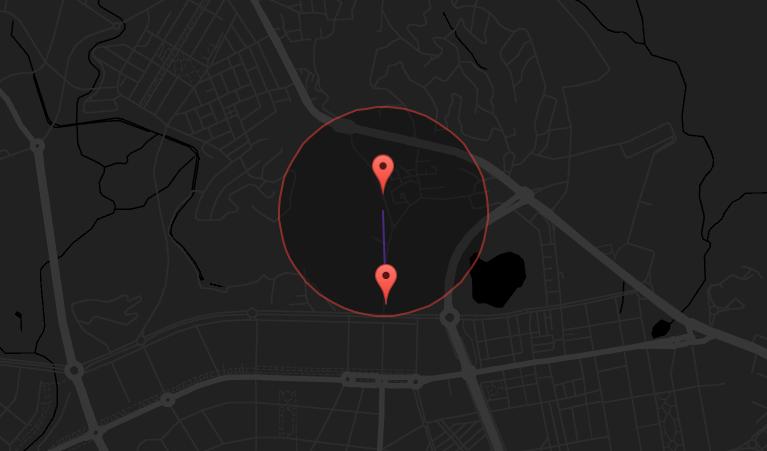
\includegraphics[width=0.7\textwidth]{graphs/pruebaLocalizacion}
	\caption{Posici�n del concentrador y nodo durante la prueba en el punto de m�ximo alcance}
	\label{fig:pruebaLocalizacion}
\end{figure}

\subsection{Metodolog�a}

C�mo se ha indicado anteriormente, el concentrador se ha ubicado en un punto fijo que estuviera elevado, por ello se ha situado en el balc�n de la 2� planta de un edificio. Y el nodo se ha ido cambiado de posici�n hasta llegar a la distancia m�xima y que este perdiera la conexi�n con el concentrador, despu�s de esto se ha vuelto a acercar para comprobar la reconexi�n a la red.

\subsection{Resultados}

Despu�s de realizar las pruebas se ha estimado la distancia m�xima a la que el nodo puede situarse para poder mantener la conexi�n que es de 400m, pero esta medida mejorar�a cambiando la antena y utilizando un amplificador en transmisi�n lo que quedar� como una l�nea futura de mejora de este proyecto.\\

En cuanto a la reconexi�n del nodo, ha sido todo un �xito. Despu�s de repetir la desconexi�n y reconexi�n del nodo var�as veces, en todas de ellas la ha realizado sin problemas. Y adem�s no ha dejado de enviar los mensajes de la web f�sica en ning�n momento durante la prueba.\\
\begin{figure}[h]
	\centering
	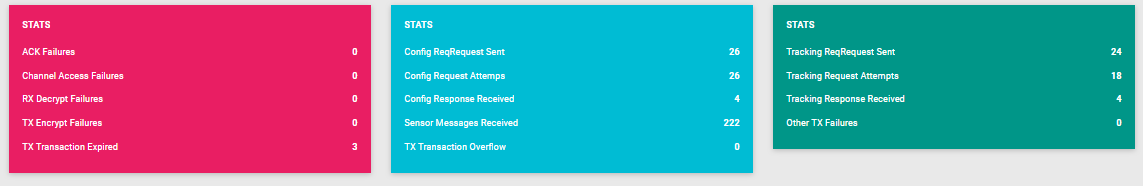
\includegraphics[width=\textwidth]{graphs/pruebaEstadisticas}
	\caption{Estad�sticas de la red despu�s de la prueba}
	\label{fig:pruebaEstadisticas}
\end{figure}
Finalmente en la figura \ref{fig:pruebaEstadisticas} se observan las estad�sticas que ha recogido la red despu�s de las pruebas,  donde se tiene que el concentrador ha recibido 26 peticiones del nodo para que le env�e la configuraci�n (esta petici�n se realiza despu�s de una conexi�n o reconexi�n)  y 222 mensajes de tipo "Sensor" que son los que el nodo env�a peri�dicamente con datos de temperatura, bater�a, estad�sticas y algunos par�metros m�s.

\section{Prueba de consumo}
\subsection{Introducci�n}
Para una exitosa implementaci�n del \ac{IOT} uno de los requisitos m�s importantes es un consumo eficiente del sistema.\\

La comunicaci�n inal�mbrica entre los nodos comienza a ser un problema cuando la fuente de alimentaci�n es limitada. Un sistema que pueda funcionar con una sola pila AAA durante a�os es lo ideal en el \ac{IOT} \cite{mahmoud2016study}. Por ello, durante el desarrollo de este proyecto se ha utilizado como protocolo inal�mbrico el IEEE 802.15.4, que destaca su bajo consumo.\\

\subsection{Medida del consumo}

Para realizar la medida de consumo se ha utilizado el mult�metro digital Keysight 34411A, que proporciona 6 d�gitos y medio de resoluci�n o una velocidad de muestreo de 50000 muestras/s a una resoluci�n inferior. \cite{multimeter4411A}\\

Para el control del mult�metro se ha utilizado dos programas de LabView, uno de ellos permite obtener datos a la m�xima velocidad de muestreo aunque eso limite la resoluci�n a 4 d�gitos (figura \ref{fig:capturaRapida}) y el otro programa permite tomar datos promediados en intervalos de tiempo (figura \ref{fig:capturaPromedio}).

\begin{figure}[H]
	\centering
	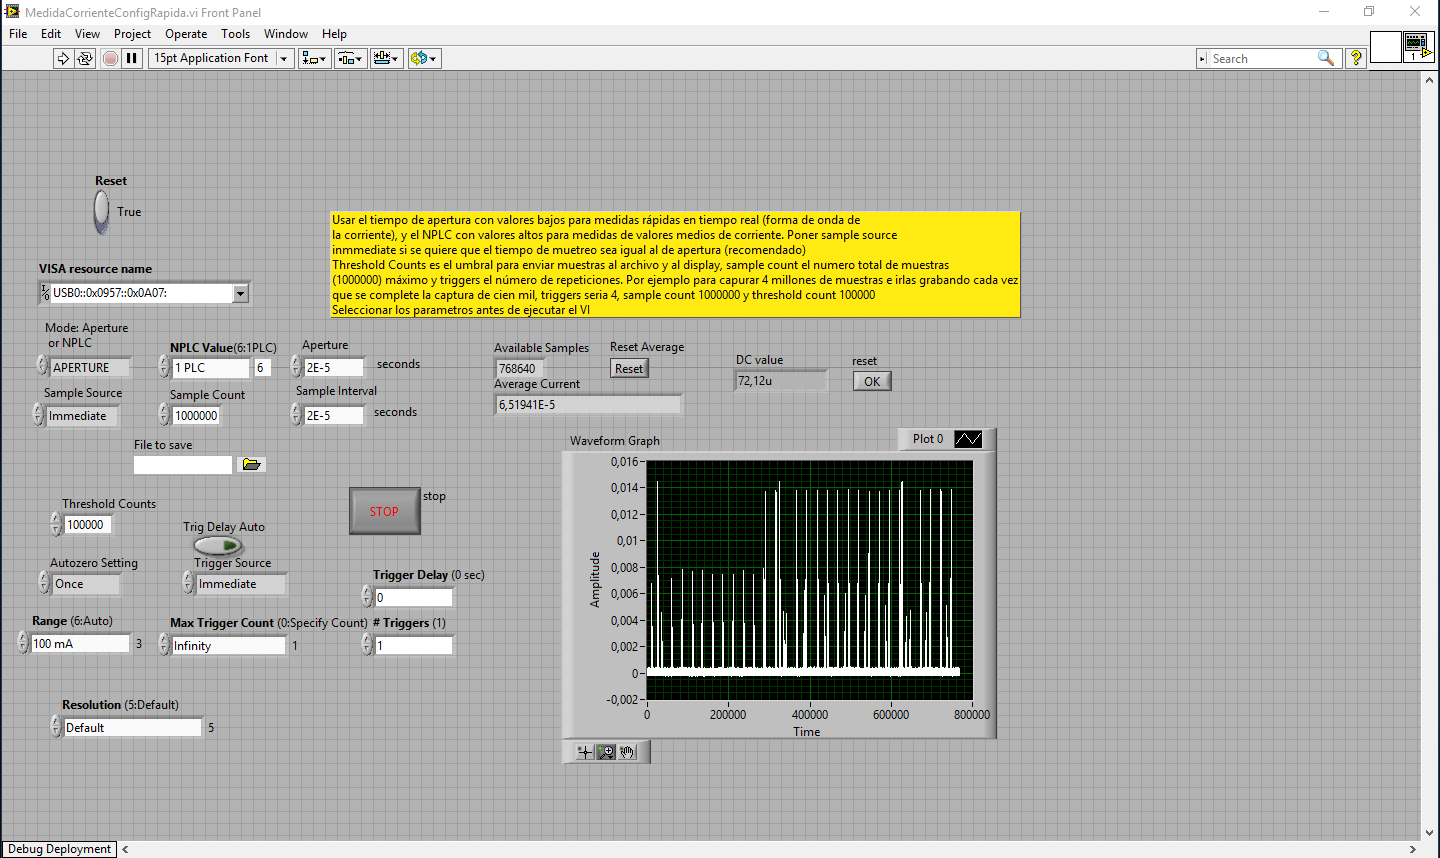
\includegraphics[width=0.8\textwidth]{graphs/CapturaRapida.png}
	\caption{Programa de LabView para captura r�pida}
	\label{fig:capturaRapida}
\end{figure}

\begin{figure}[H]
	\centering
	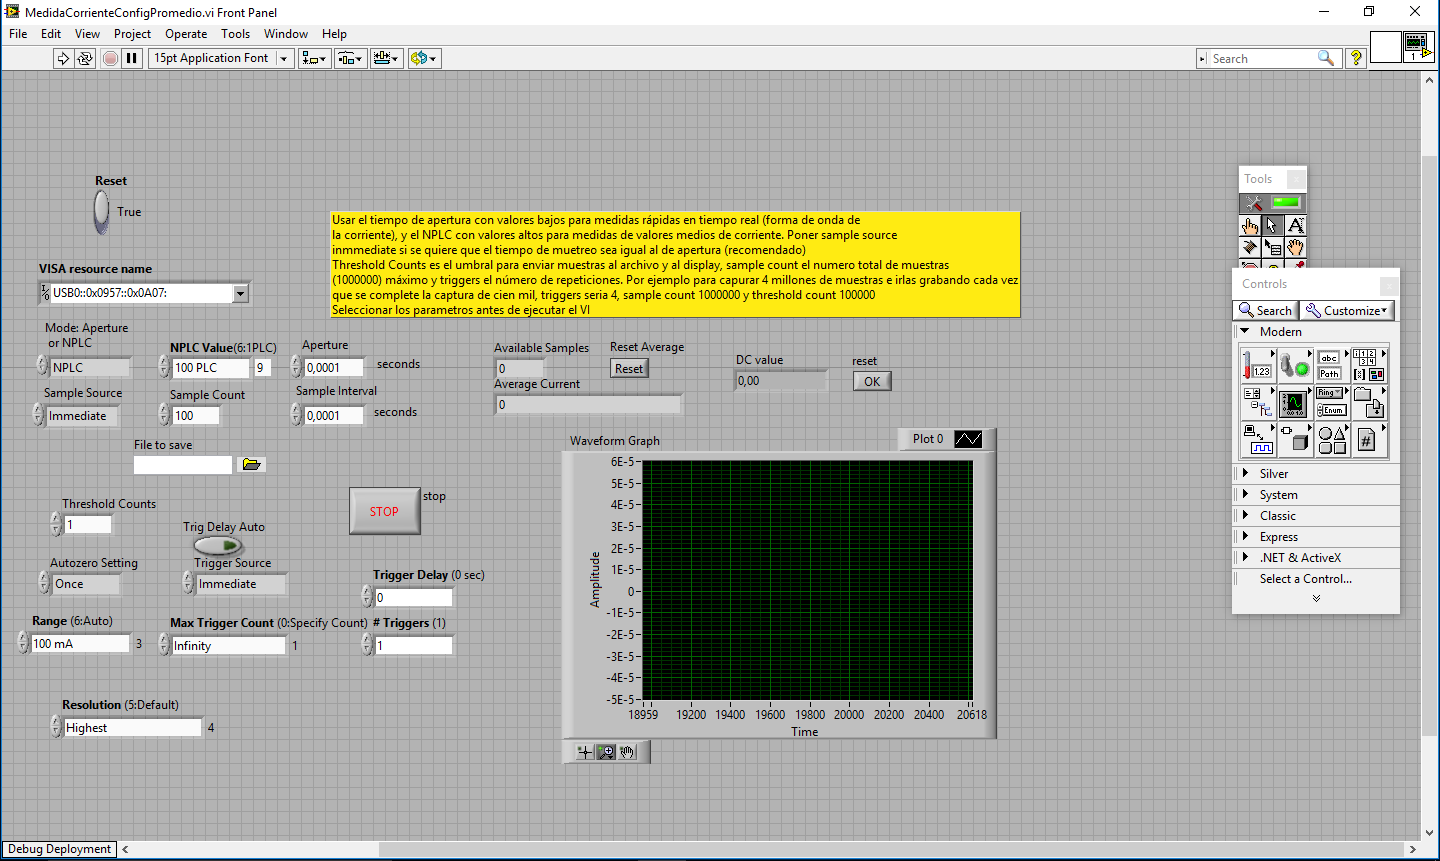
\includegraphics[width=0.8\textwidth]{graphs/CapturaPromedio.png}
	\caption{Programa de LabView para captura en promedio}
	\label{fig:capturaPromedio}
\end{figure}

\subsection{Resultados}

Aunque el objetivo de esta prueba es conocer el consumo medio de corriente del nodo. Antes de nada se necesita conocer que fondo de escala utilizar en el mult�metro para la medida en promedio, para ello se hace uso del programa de captura a m�xima frecuencia de muestreo, donde se obtiene la corriente instant�nea m�xima que consume el nodo, unos 15 mA (figura \ref{fig:datosCapturaRapida}).

\begin{figure}[h]
	\centering
	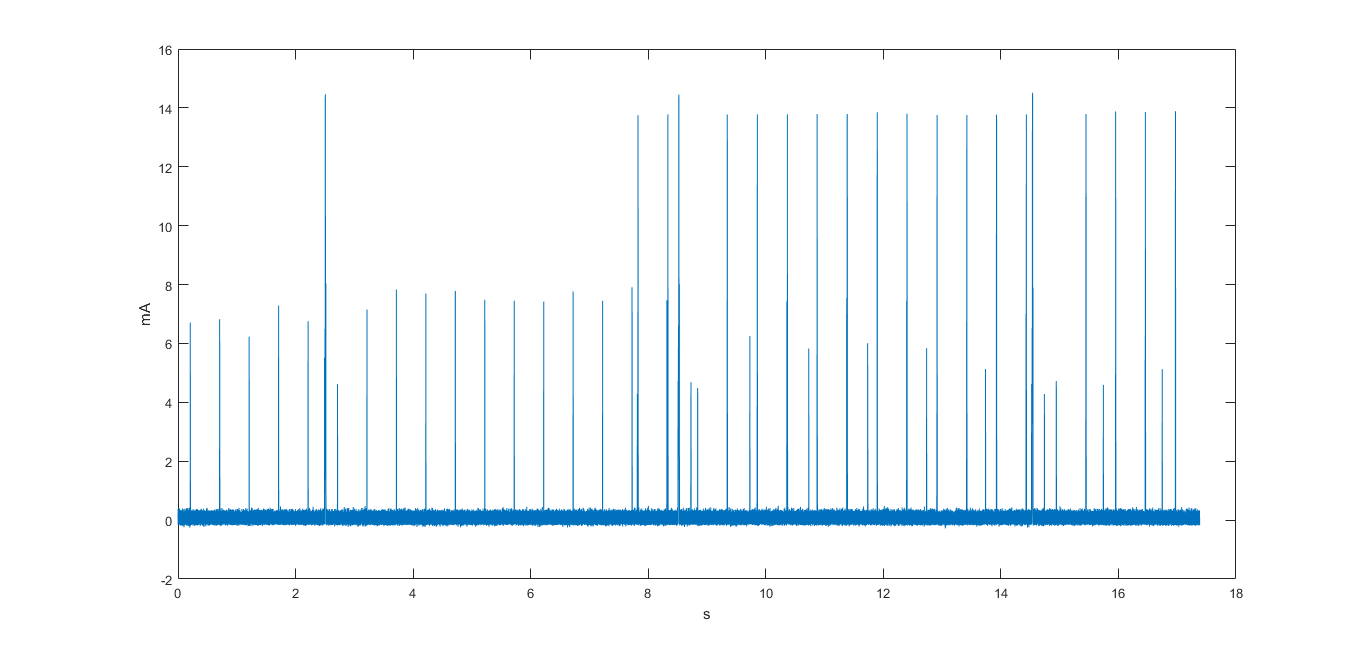
\includegraphics[width=\textwidth]{graphs/capturaRapidaDatos.png}
	\caption{Consumo en mA del nodo a la m�xima frecuencia de muestreo}
	\label{fig:datosCapturaRapida}
\end{figure}

Finalmente, utilizando el programa de medida promediada de LabView con un fondo de escala de 100mA, realizamos una medida de la corriente promedio durante 50 ciclos de subidas al servidor. Con esta configuraci�n se obtiene que el consumo medio de un nodo es de 169.6 $\micro A$, lo que equivale a m�s de 5 meses de funcionamiento utilizando una pila de bot�n CR 2477. 



\chapterend{}


\part{Conclusiones y lineas futuras}
\chapterbeginx{Conclusiones y l�neas futuras}

\sectionx{Conclusiones}
	Despu�s de todo el desarrollo del proyecto, es pertinente hacer una valoraci�n final del mismo, respecto a los resultados obtenidos, las expectativas o el resultado de la experiencia acumulada.

	En esta secci�n se exponen todos esos conceptos y enuncian unas conclusiones finales.
	
	Adem�s, considerando tambi�n el estado de la t�cnica, se pueden deducir l�neas futuras de trabajo, proponer otros puntos de vista o cualquier otra sugerencia como post�mbulo del presente trabajo, para ser considerada por el lector o el tribunal evaluador.

\sectionx{L�neas futuras}

\begin{flushright}
{\large \pfcauthorname}\nli
\today
\end{flushright}
	
\chapterend
\chapterbeginx{L�neas futuras}

Durante el desarrollo del \ac{TFG}  se ha observado un crecimiento en el uso de las tecnolog�as que implementa este proyecto, lo que vaticina un futuro donde el concepto de web f�sica sea familiar a la poblaci�n. De este crecimiento se extraen lineas futuras de desarrollo en este �mbito como son:

\begin{itemize}
	\item Mejora del alcance analizando las diferentes alternativas que ofrece TI 15.4-Stack.
	\item Crear un nodo que emule una m�quina expendedora, donde el usuario pueda realizar su compra a trav�s de la web f�sica.
	\item Mejora de la duraci�n de la bater�a optimizando el c�digo y a�adiendo tecnolog�a de recolecci�n de energ�a.
	\item Creaci�n de placas de circuito impreso para nodo y concentrador que permita reducir el tama�o.
\end{itemize}


\begin{flushright}
{\large \pfcauthorname}\nli
\today
\end{flushright}
	
\chapterend{}
% Anexos
\part{Ap�ndices}

\appendix

\pagestyle{fancy}
\fancyhead[LE,RO]{\thepage}
\fancyhead[RE]{Ap�ndice} %
\fancyhead[LO]{\nouppercase{\rightmark}}
%\fancyhead[RE]{Parte \thepart \rightmark} %

\chapter{Estructuras de mensajes OTA}
\label{apd:estructurasMensajes}

Em la figura \ref{fig:mensajesSMSGS} se observan los distintos tipos de mensajes que se env�an sobre la red inal�mbrica, estos mensajes est�n definidos en el fichero \textit{smsgs.h}

\begin{figure}[H]
	\centering
	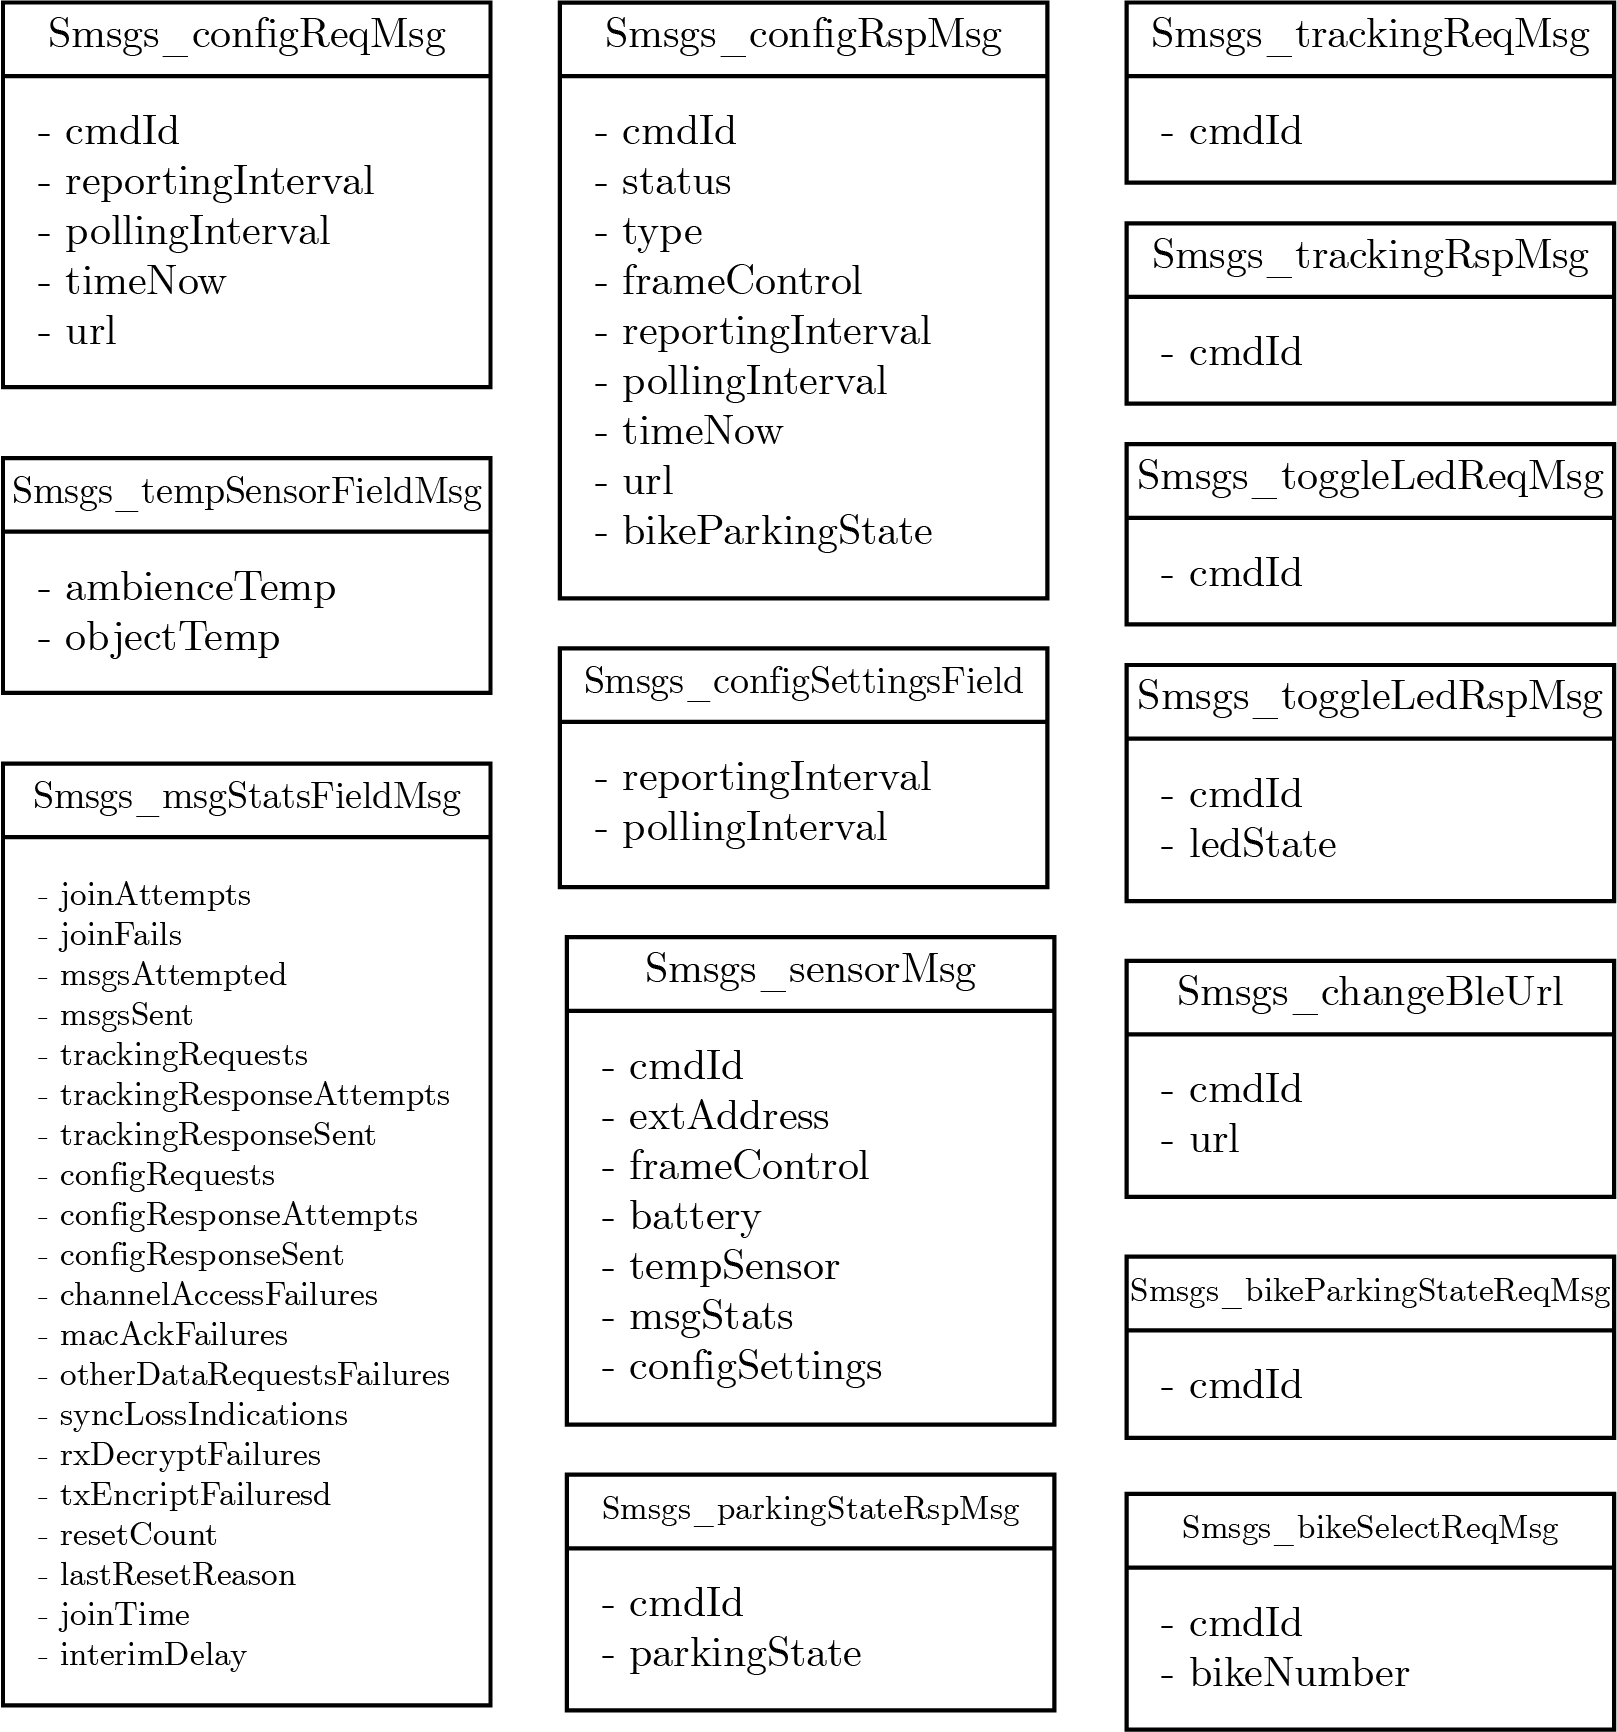
\includegraphics[width=\textwidth]{graphs/mensajesSMSGS}
	\caption{Estructuras de los mensajes del fichero smsgs.h}
	\label{fig:mensajesSMSGS}
\end{figure}


\pagestyle{fancy}
\fancyhead[LE,RO]{\thepage}
\fancyhead[RE]{Ap�ndice} %
\fancyhead[LO]{\nouppercase{\rightmark}}
%\fancyhead[RE]{Parte \thepart \rightmark} %

\chapter{Herramientas utilizadas}
\label{apd:herramientasUtilizadas}

\begin{center}
	\begin{longtable}{ m{0.3\textwidth} p{0.7\textwidth} }
		
\includegraphics[align=t,width=0.2\textwidth]{graphs/logo-github}& 
		GitHub es una plataforma para alojar proyectos utilizando el sistema de control de versiones GIT.
		\\ 
		\hline
		 
\includegraphics[align=t,width=0.2\textwidth]{graphs/logo-aws} &  
		 \textit{Amazon Web Services} (AWS) es una colecci�n de servicios web que conjunto forman una plataforma de computaci�n en la nube.
		  \\ 
		  \hline
		   
\includegraphics[align=t,width=0.2\textwidth]{graphs/logo-texStudio} &  
		  TeXstudio es un entorno de escritura intregrado para crear documentos LaTeX.
		  \\ 
		  \hline
		  
		  
\includegraphics[align=t,width=0.2\textwidth]{graphs/logo-latex} &  
		  LaTeX es un sistema de composici�n de textos, orientado a la creaci�n de documentos escritos que presenten una alta calidad tipogr�fica.
		  \\ 
		  \hline
		  
		  
\includegraphics[align=t,width=0.2\textwidth]{graphs/logo-illustrator} &  
		  Adobe Illustrator es un editor de gr�ficos vectoriales y est� destinado a la creaci�n art�stica de dibujo y pintura para ilustraci�n. 
		  \\ 
		  \hline
		  
		  
\includegraphics[align=t,width=0.2\textwidth]{graphs/logo-sublime} &  
		  Sublime text es un editor de texto y editor de c�digo fuente.
		  \\ 
		  \hline
		  
		  
\includegraphics[align=t,width=0.2\textwidth]{graphs/logo-node} &  
		  Node.js es un entrono de ejecuci�n para JavaScript construido con el motor de JavaScript V8 de Chrome. 
		  \\ 
		  \hline
		  
		  
\includegraphics[align=t,width=0.2\textwidth]{graphs/logo-angular} &  
		  AngularJS es un \textit{framework} de JavaScript de c�digo abierto, mantenido por Google, que se utiliza para crear y mantener aplicaciones web de una sola p�gina.
		  \\ 
		  \hline
		  
		  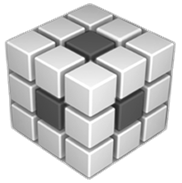
\includegraphics[align=t,width=0.2\textwidth]{graphs/logo-ccs} &  
		  Code Composer Studio es un entorno integrado de desarrollo que soporta los microcontroladores de Texas Instruments. 
		  \\ 
		  \hline
		  
		  
\includegraphics[align=t,width=0.2\textwidth]{graphs/logo-mongo} &  
		  MongoDB es una base de datos NoSQL orientado a documentos, desarrollado bajo el concepto de c�digo abierto.
		  \\ 
		  \hline
		  
		  
\includegraphics[align=t,width=0.2\textwidth]{graphs/logo-raspbian} &  
		  Raspbian es un distribuci�n del sistema operativo GNU/Linux y basado en Debian Jessie para la Raspberry Pi.
		  \\ 
		  \hline
		  
		  
\includegraphics[align=t,width=0.2\textwidth]{graphs/logo-express} &  
		  Express es una infraestructura de aplicaciones web Node.js m�nima y flexible que proporciona un conjunto s�lido de caracter�sticas para las aplicaciones web y m�viles.
		  \\ 
		  \hline

	\end{longtable} 
\end{center}

\chapterend

\chapterbegin{Funcionamiento}
\label{chp:funcionamiento}
\minitoc

\sectionx{Inicio de la red}


\subsection*{1. Iniciar el servidor}

El primer paso es iniciar el servidor, ya que toda la red depende de este. Como se ha utilizado Amazon Web Services, desde su web iniciamos la instancia que corre en el inicio el servidor de la aplicaci�n (v�ase figura \ref{fig:screenAWS}.

\begin{figure}[h]
	\centering
	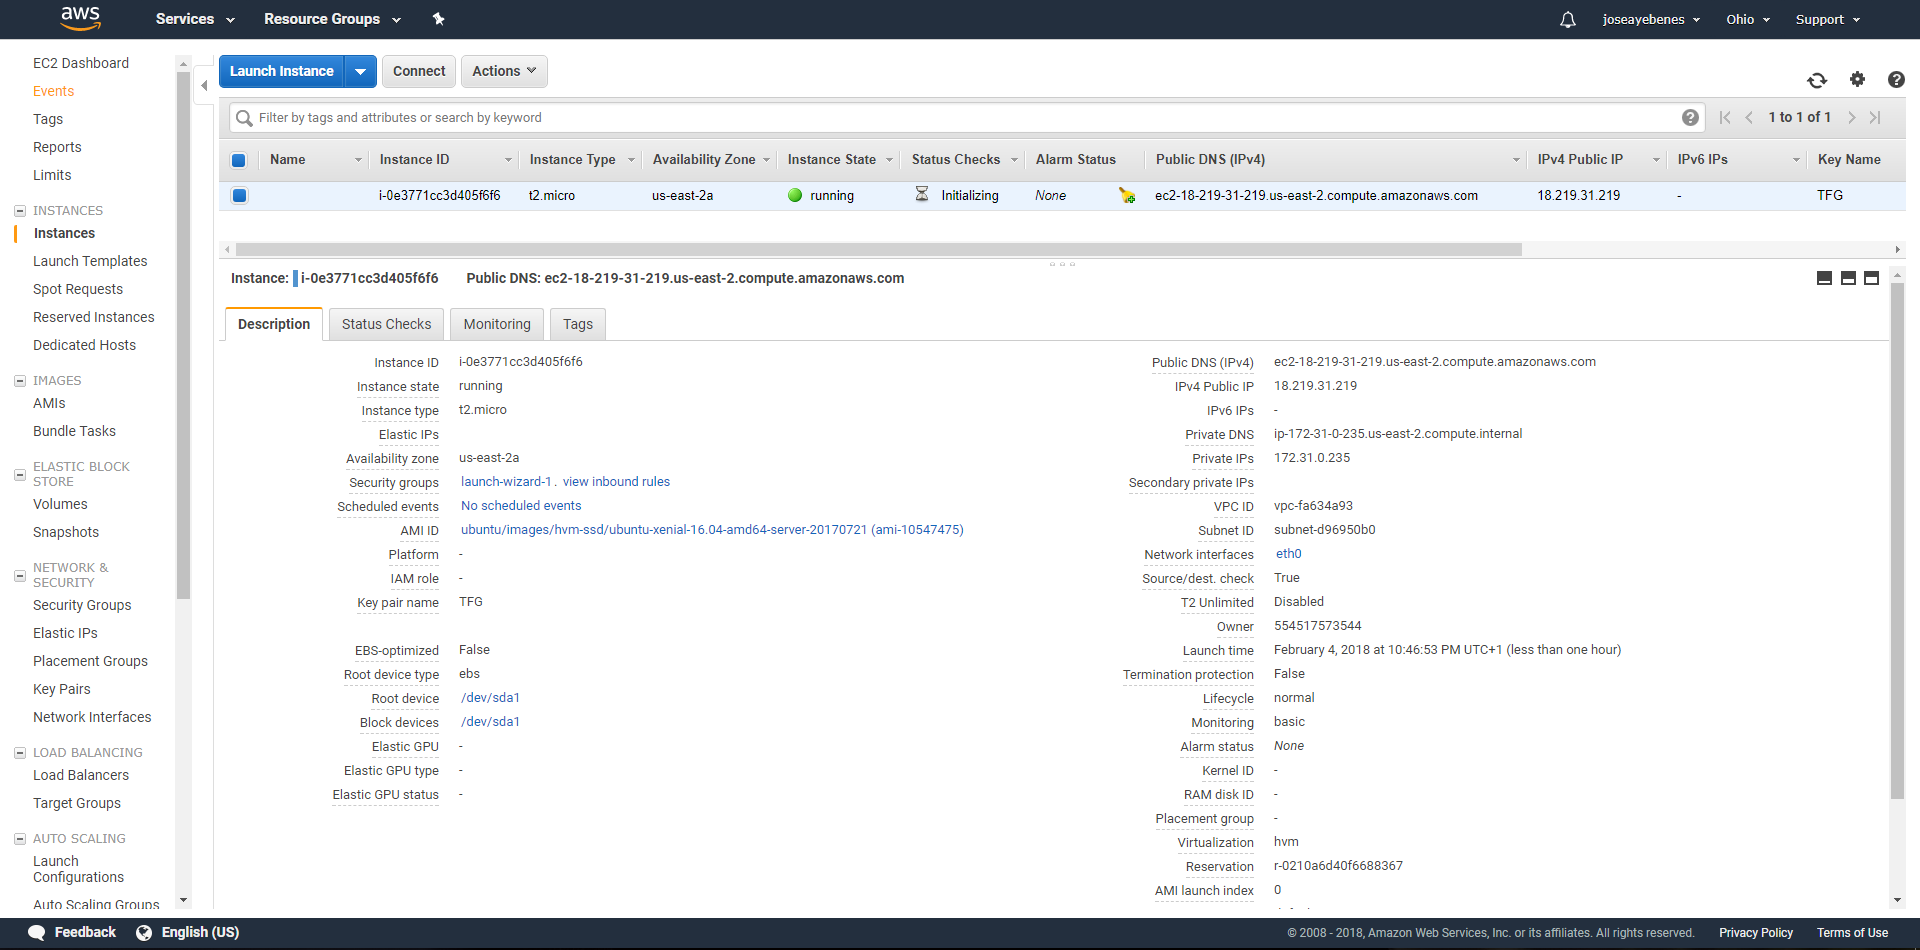
\includegraphics[width=\textwidth]{graphs/screenAWS.PNG}
	\caption{Web de gesti�n de instancias en Amazon Web Services}
	\label{fig:screenAWS}
\end{figure}

Despu�s de iniciar el servidor, es posible acceder a la web de gesti�n desde la direcci�n dns de la instancia del servidor en el puerto 5000. Inicialmente el concentrador no est� conectado por lo que nos aparece un mensaje indic�ndolo, figura \ref{fig:screenWebNotConnected}.

\begin{figure}[h]
	\centering
	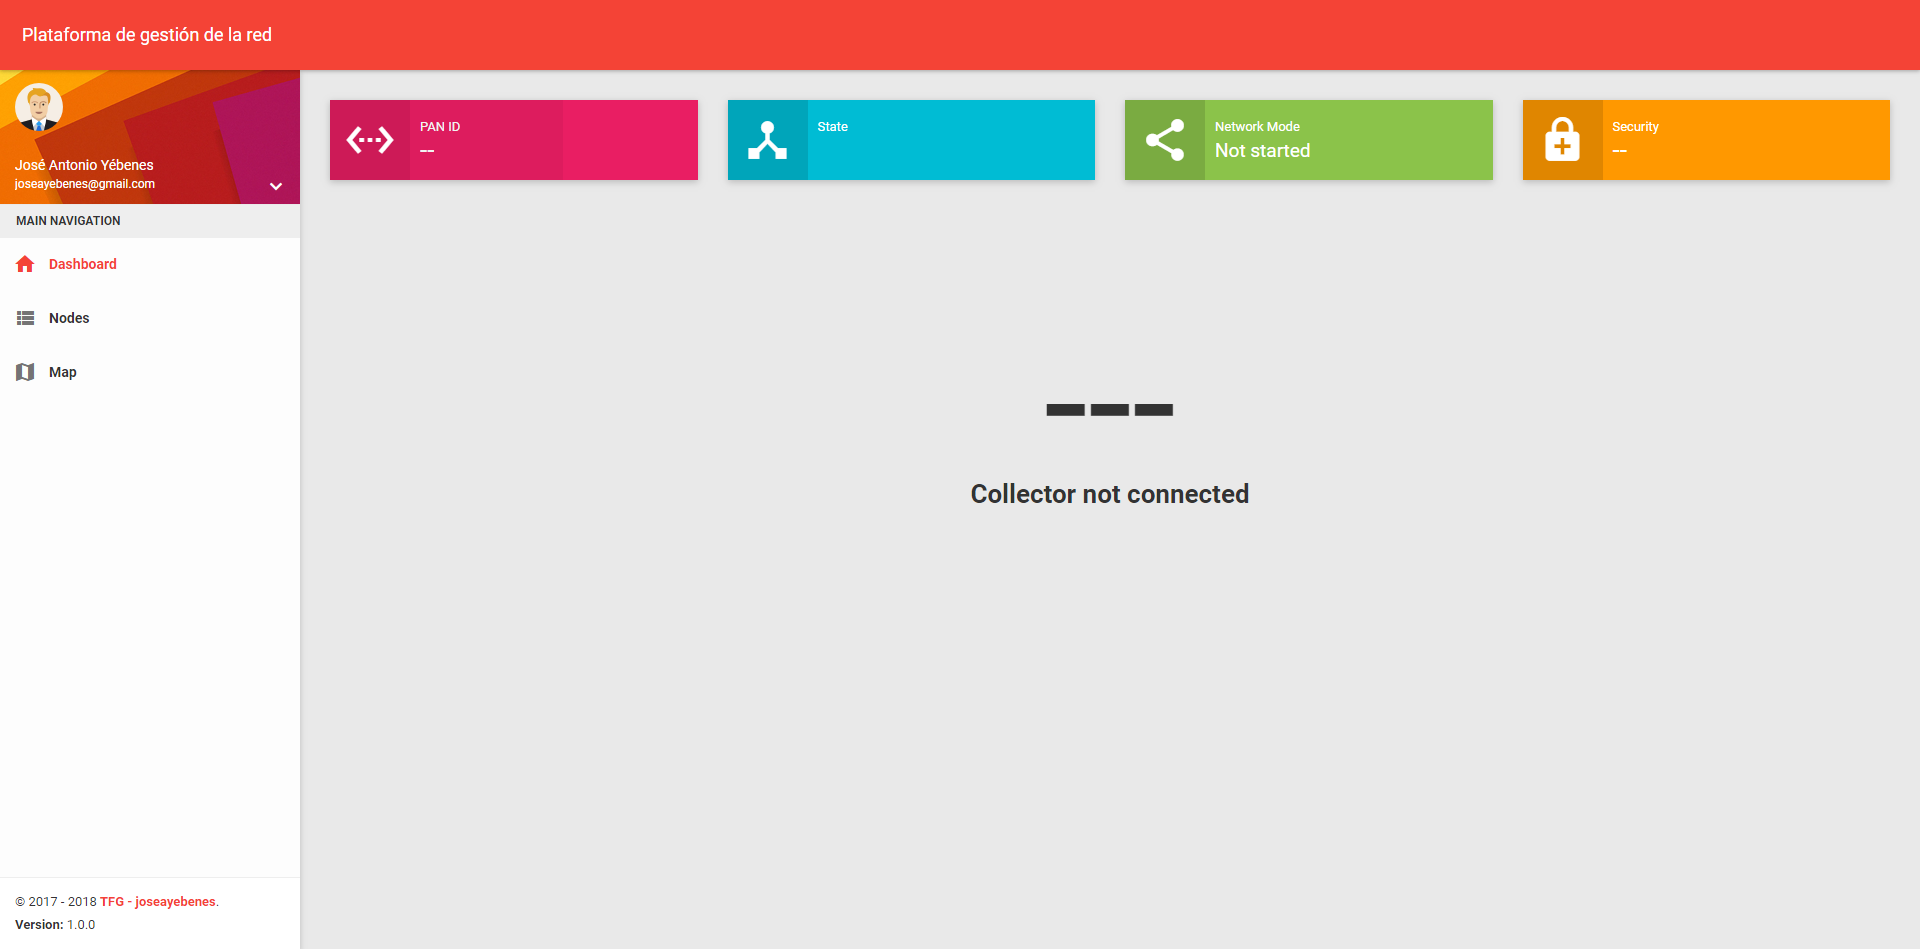
\includegraphics[width=\textwidth]{graphs/screenWebNotConnected.PNG}
	\caption{Apariencia de la web cuando no est� conectado el concentrador}
	\label{fig:screenWebNotConnected}
\end{figure}

\subsection*{2. Encender concentrador}

Antes de enceder la RaspberryPi, conectamos el coprocesador por USB y damos conexi�n a Internet a la RaspberryPi. La RaspberryPi est� configurada para ejecutar el programa del concentrador y conectarse al servidor, por lo que no es necesaria m�s interacci�n con el concentrador. Despu�s de encenderse la RaspberryPi, la web habr� cambiado y ahora ya nos indicar� algunos par�metros de la web, figura \ref{fig:screenWebConnected}.\\

En la parte superior de la web se observan los par�metros de la red como son su direcci�n PAN, el estado que indica si la red permite la conexi�n de los nodos, el tipo de comunicaci�n y si est� activada la seguridad.

\begin{figure}[H]
	\centering
	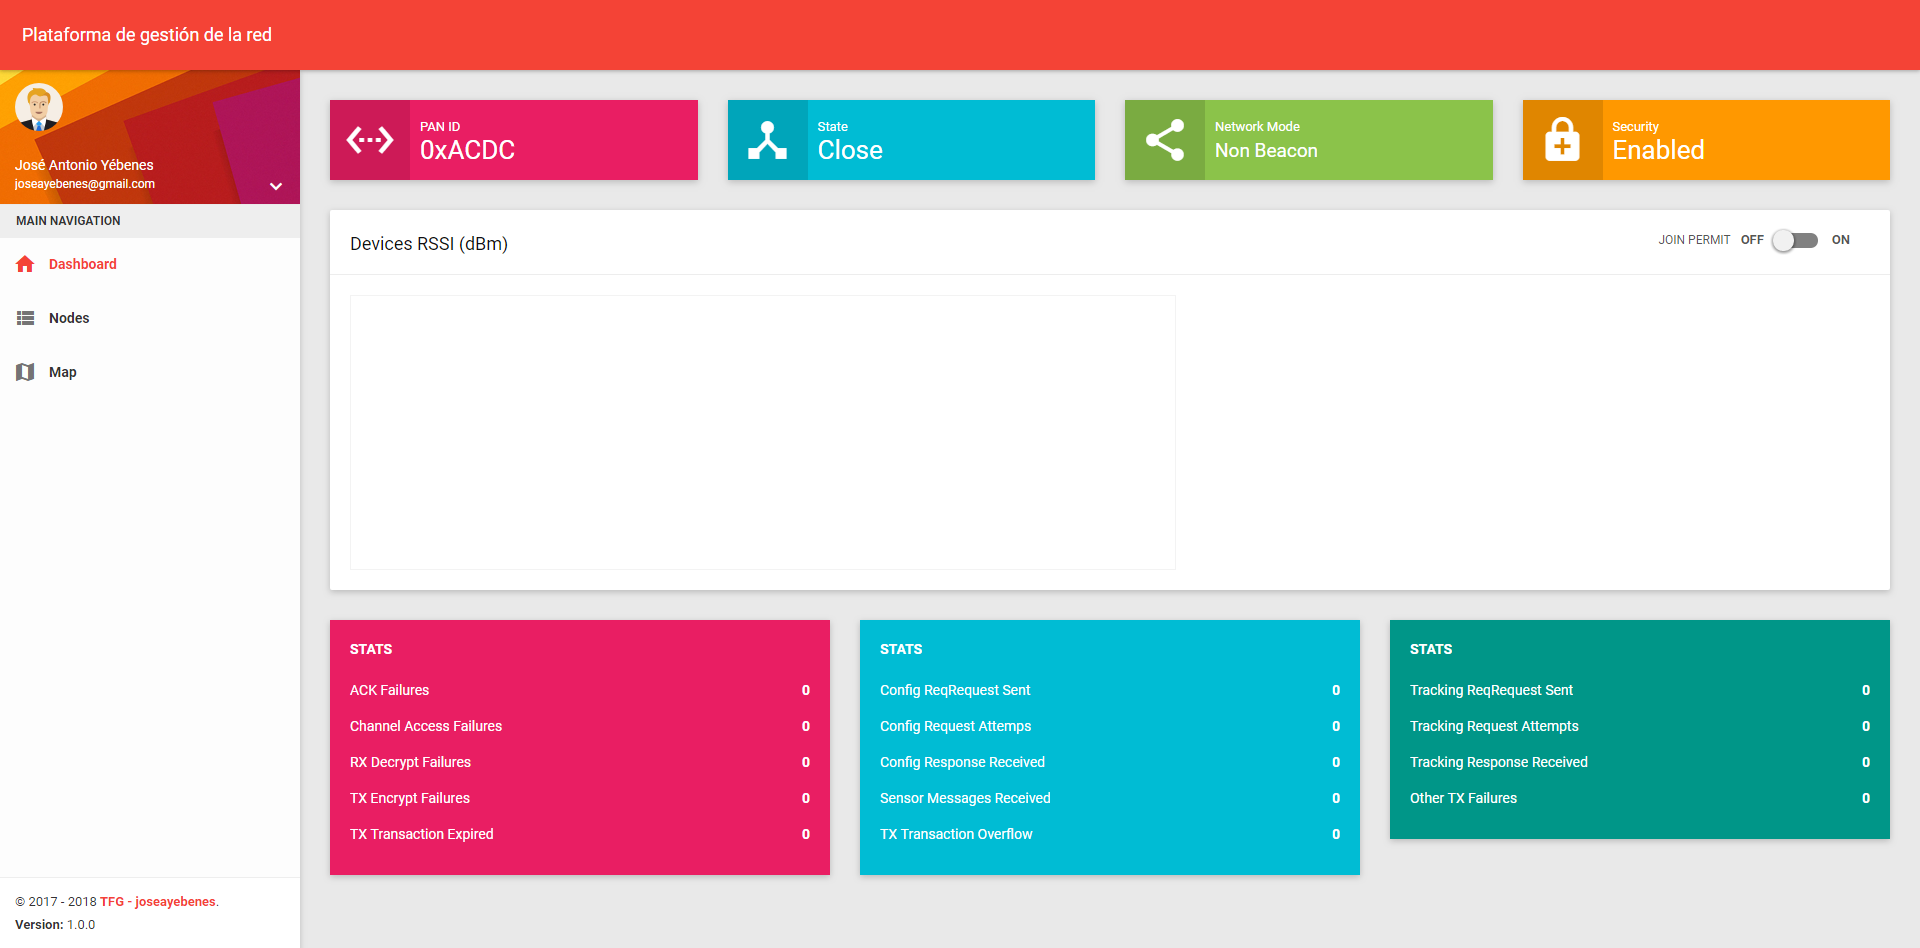
\includegraphics[width=\textwidth]{graphs/screenWebConnected.PNG}
	\caption{Apariencia de la web cuando ya est� conectado el concentrador}
	\label{fig:screenWebConnected}
\end{figure}

\subsection*{2. Encender nodos}

Encendemos todos los nodos necesarios, en las pruebas realizadas hemos utilizado dos.


\subsection*{3. Permitir conexiones de los nodos}

Para permitir la conexi�n de los nodos a la red, es necesario poner el bot�n ``\textit{JOIN PERMIT}'' a ``ON''. Despu�s de eso, los nodos que ya haya encendidos, se conectar�n a la red y aparecer�n en la web.\\

En la figura \ref{fig:screenWebConnectedOpenTwoDevices} se observa la apariencia de la web cuando dos dispositivos est� conectados.  En la parte central se observa una gr�fica con potencia de la se�al de cada uno de los nodos en dBi, y en la parte inferior estad�sticas generales de la red.

\begin{figure}[H]
	\centering
	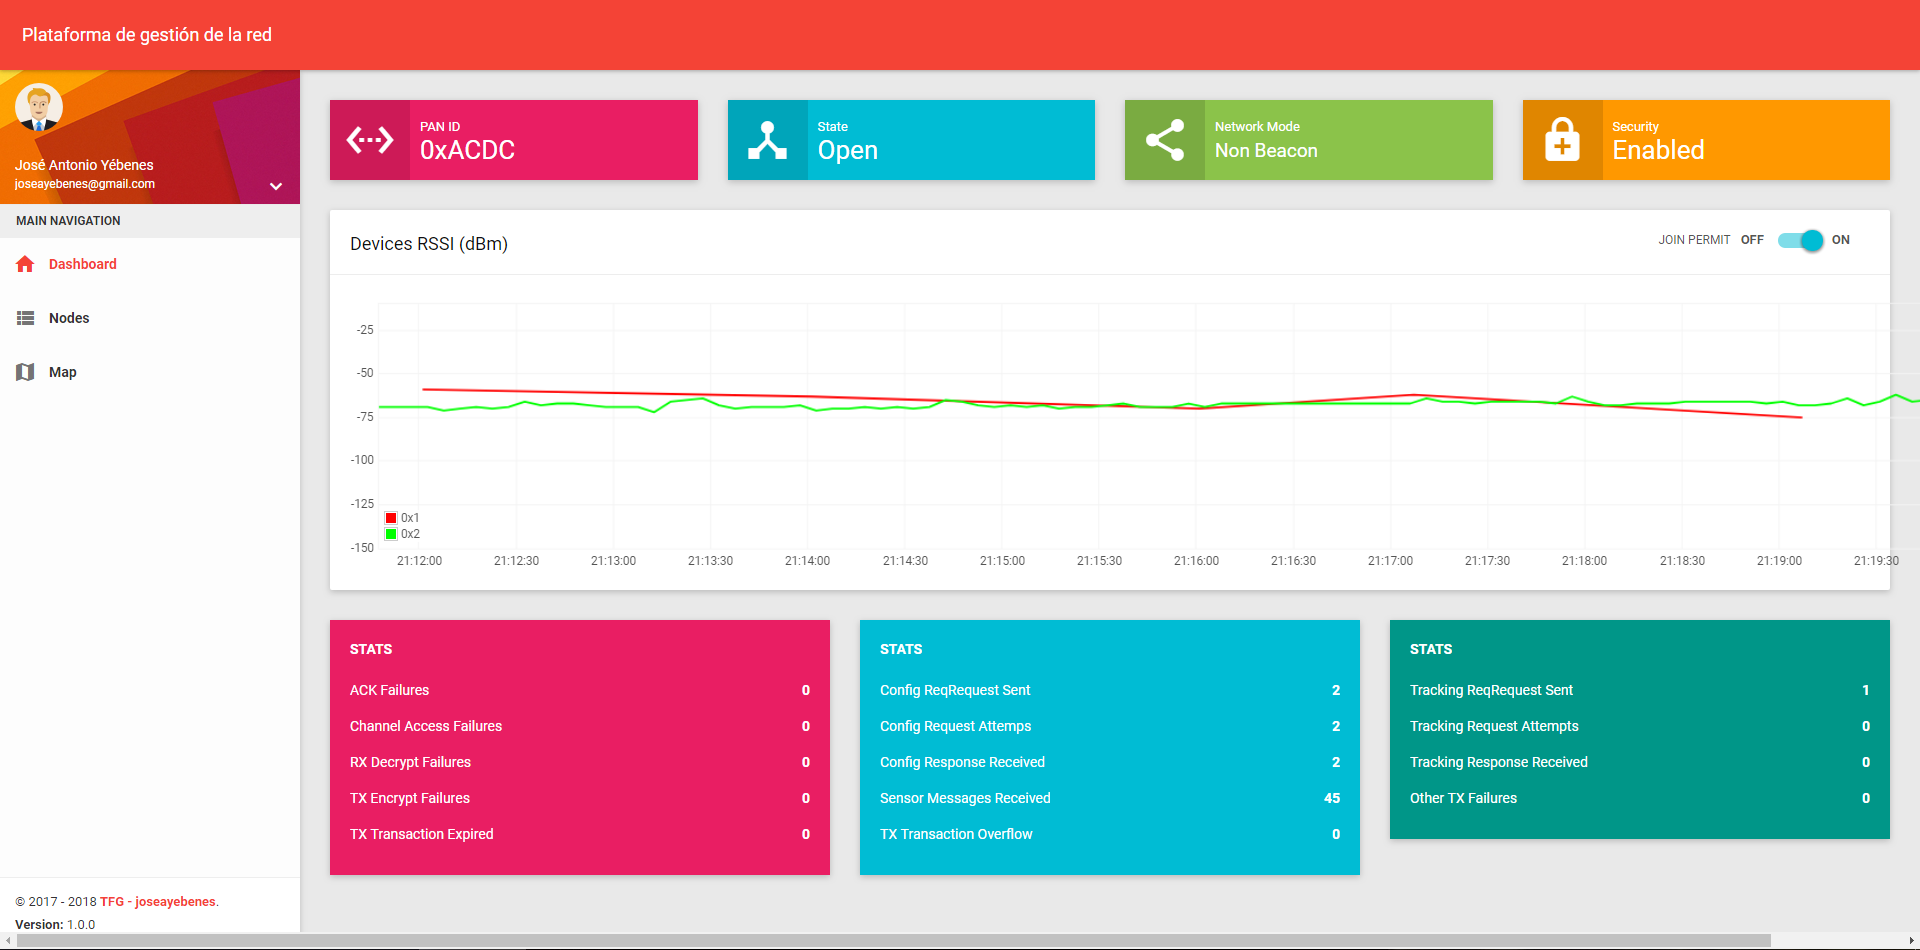
\includegraphics[width=\textwidth]{graphs/screenWebConnectedOpenTwoDevices.PNG}
	\caption{Apariencia de la web cuando hay dos nodos conectados}
	\label{fig:screenWebConnectedOpenTwoDevices}
\end{figure}

\sectionx{Administraci�n de los nodos}

Si se hace click en la barra de navegaci�n derecha en el bot�n ``\textit{Nodes}'', se accede al panel de administraci�n de los nodos, en el aparecen la lista de nodos conectados y la informaci�n relevante de cada uno, como se observa en la figura \ref{fig:screenWebNodes}.

\begin{figure}[H]
	\centering
	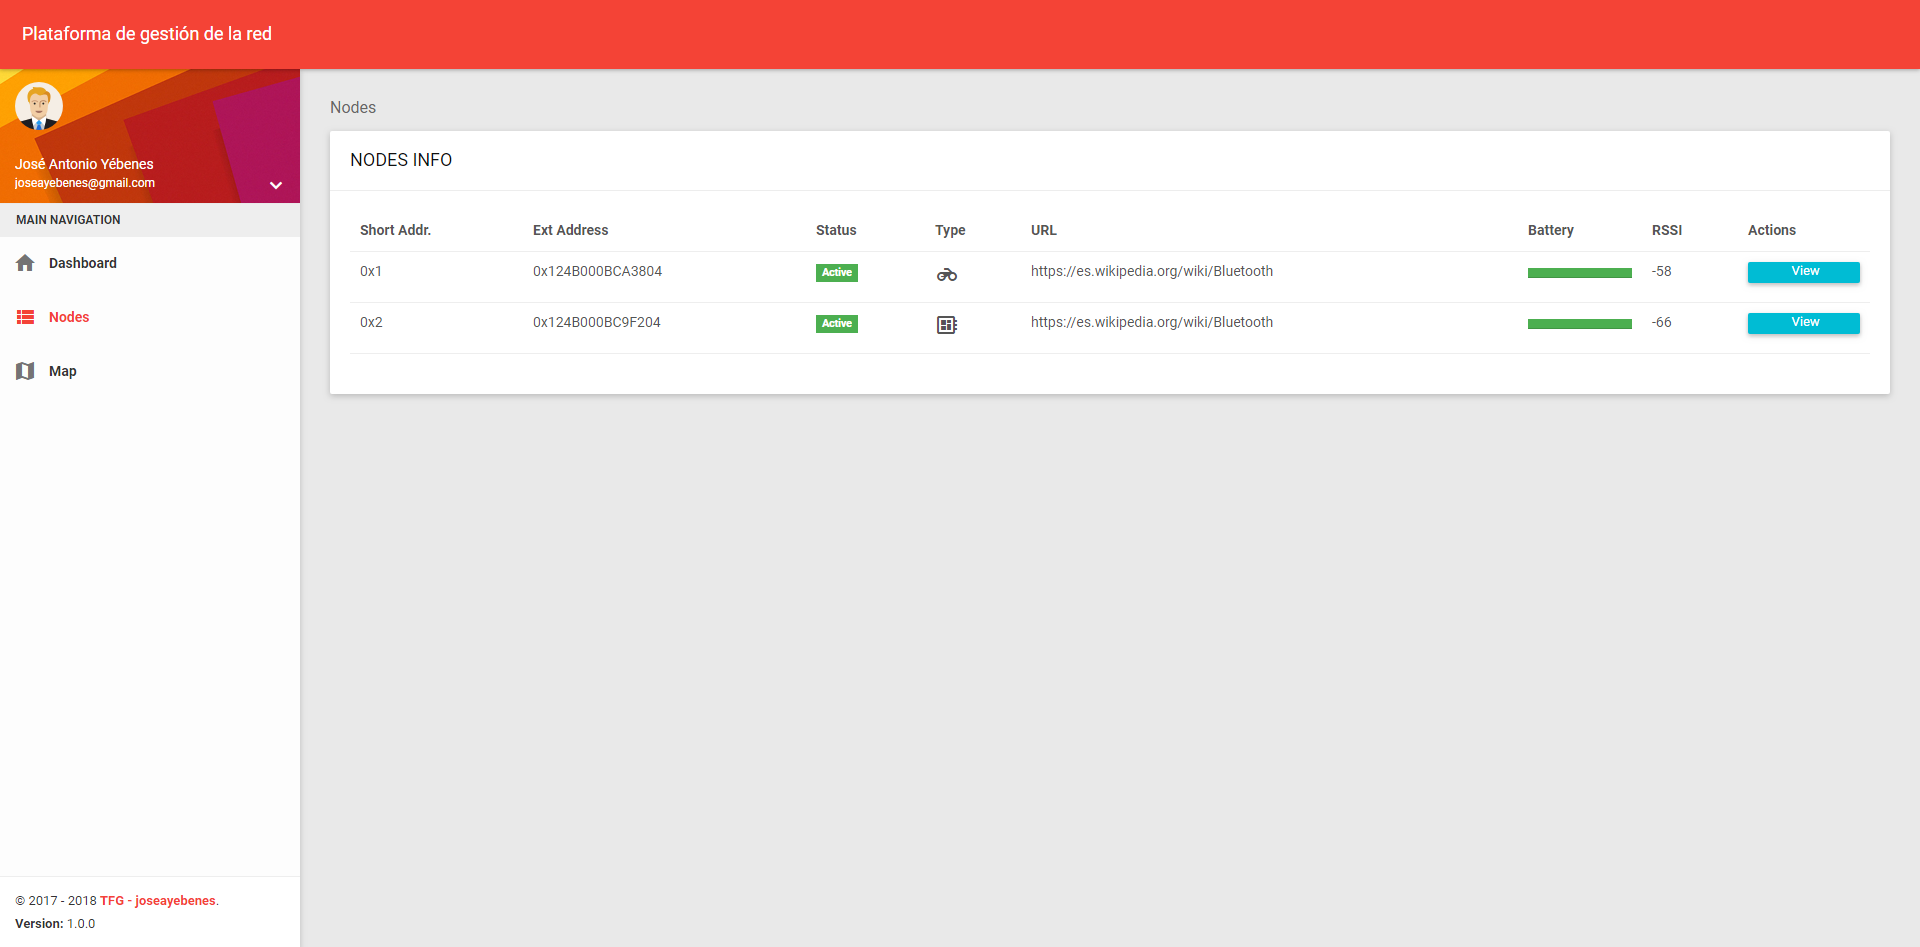
\includegraphics[width=\textwidth]{graphs/screenWebNodes.PNG}
	\caption{Panel de administraci�n de los nodos}
	\label{fig:screenWebNodes}
\end{figure}

Haciendo click en alguno de los botones ``\textit{View}'', se accede a la administraci�n del nodo correspondiente, como se aprecia en la tabla hay dos tipos de nodos, uno representado con una bicicleta y el otro con el s�mbolo de un microcontrolador, que representan un nodo destinado al control de un parking de bicicletas y un nodo gen�rico de informaci�n respectivamente. Cada tipo de nodo tiene una interfaz de administraci�n diferente.

\subsection*{Administraci�n de nodo gen�rico}

En la figura \ref{fig:screenWebNodeGenericDetails}, se puede observar toda la informaci�n relevante sobre el nodo seleccionado.\\

En el cuadro de ``\textit{Physical Web - URL}'' es posible modificar la URL que env�a dicho nodo. Justo debajo del t�tulo aparece la URL que actualmente est� enviando. En el cuadro se puede introducir cualquier URL de tipo HTTPs y al hacer click en el bot�n se enviar� el cambio al nodo.\\

Tambi�n es posible indicar cuales son las coordenadas del nodo desde el cuadro ``\textit{Position}''.

\begin{figure}[h]
	\centering
	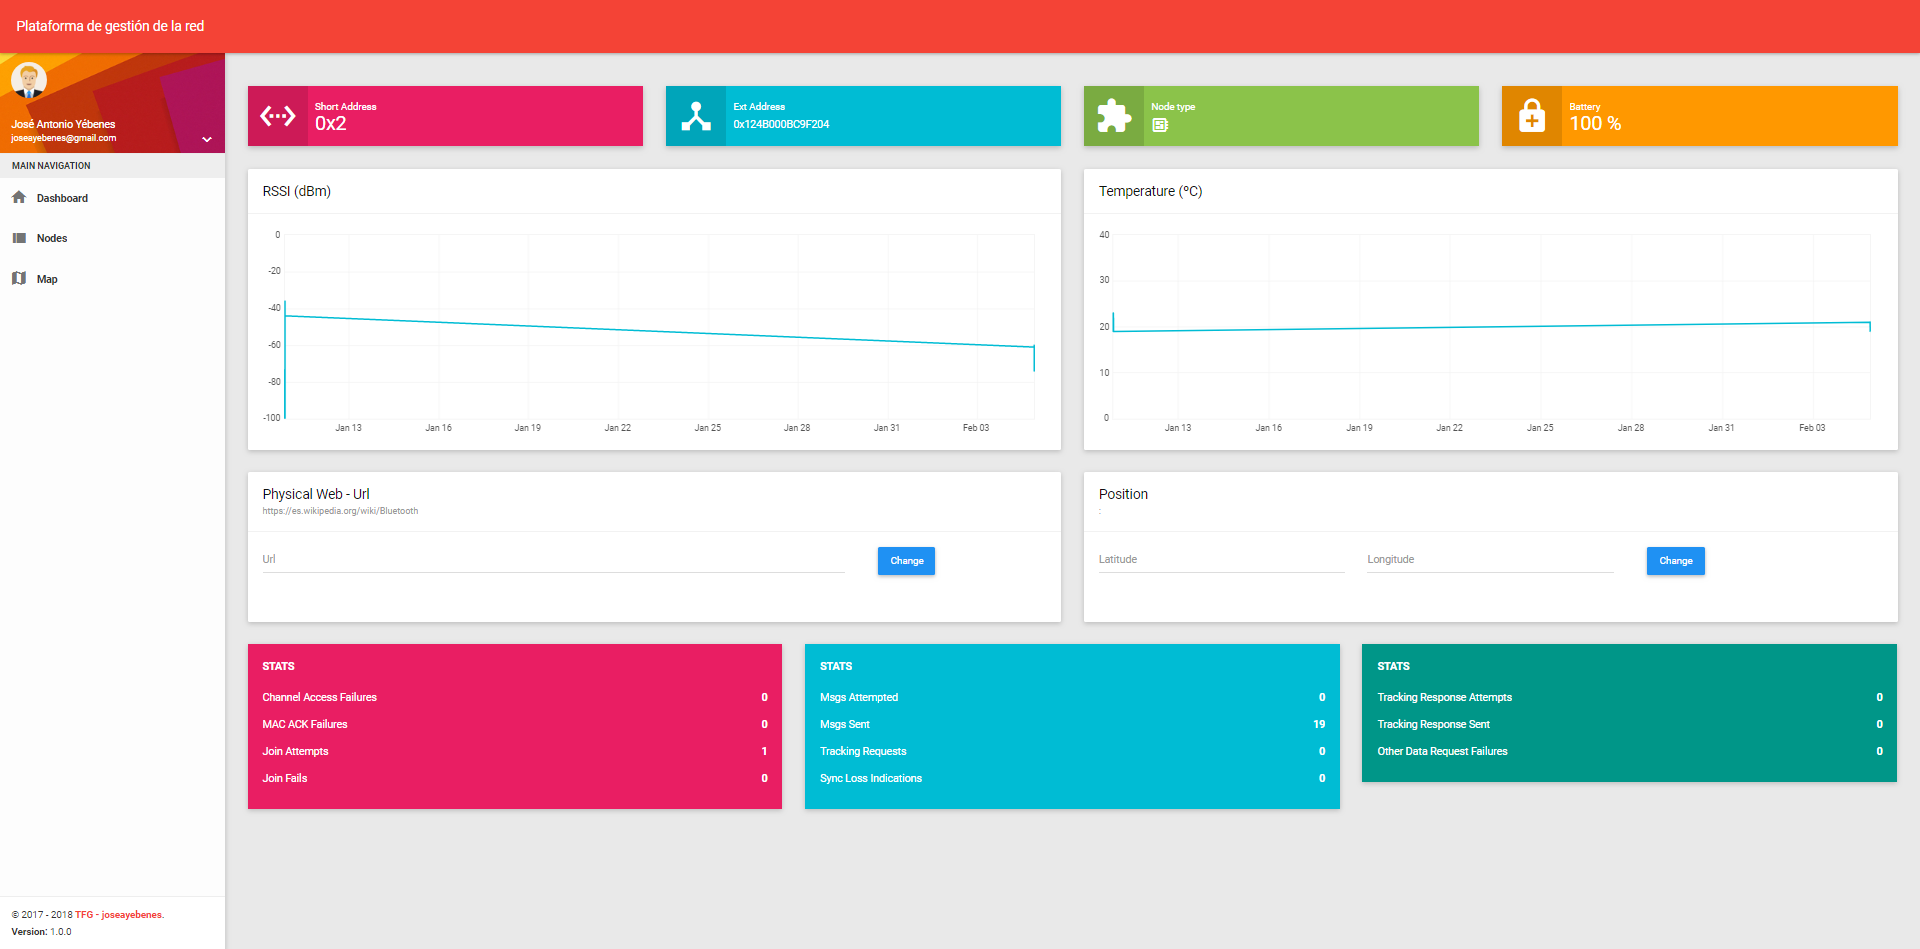
\includegraphics[width=\textwidth]{graphs/screenWebNodeGenericDetails.PNG}
	\caption{Panel de administraci�n de un nodo tipo gen�rico}
	\label{fig:screenWebNodeGenericDetails}
\end{figure}

\subsection*{Administraci�n de un tipo parking de bicicletas}

El panel de administraci�n de este tipo de nodo se observa en la figura \ref{fig:screenWebNodeBikeDetails}. Esta web permite lo mismo que la web de un nodo gen�rico, pero adem�s hay un cuadro llamado ``\textit{Parking}'', en este cuadro se observar�a el estado de cada anclaje del parkin, y si se hace click en cualquiera de ellos el estado del anclaje cambiar�a de abierto a cerrado o vicerversa. Esta funci�n est� simulada en el nodo como un array donde se guardan los estados de los candados.

\begin{figure}[H]
	\centering
	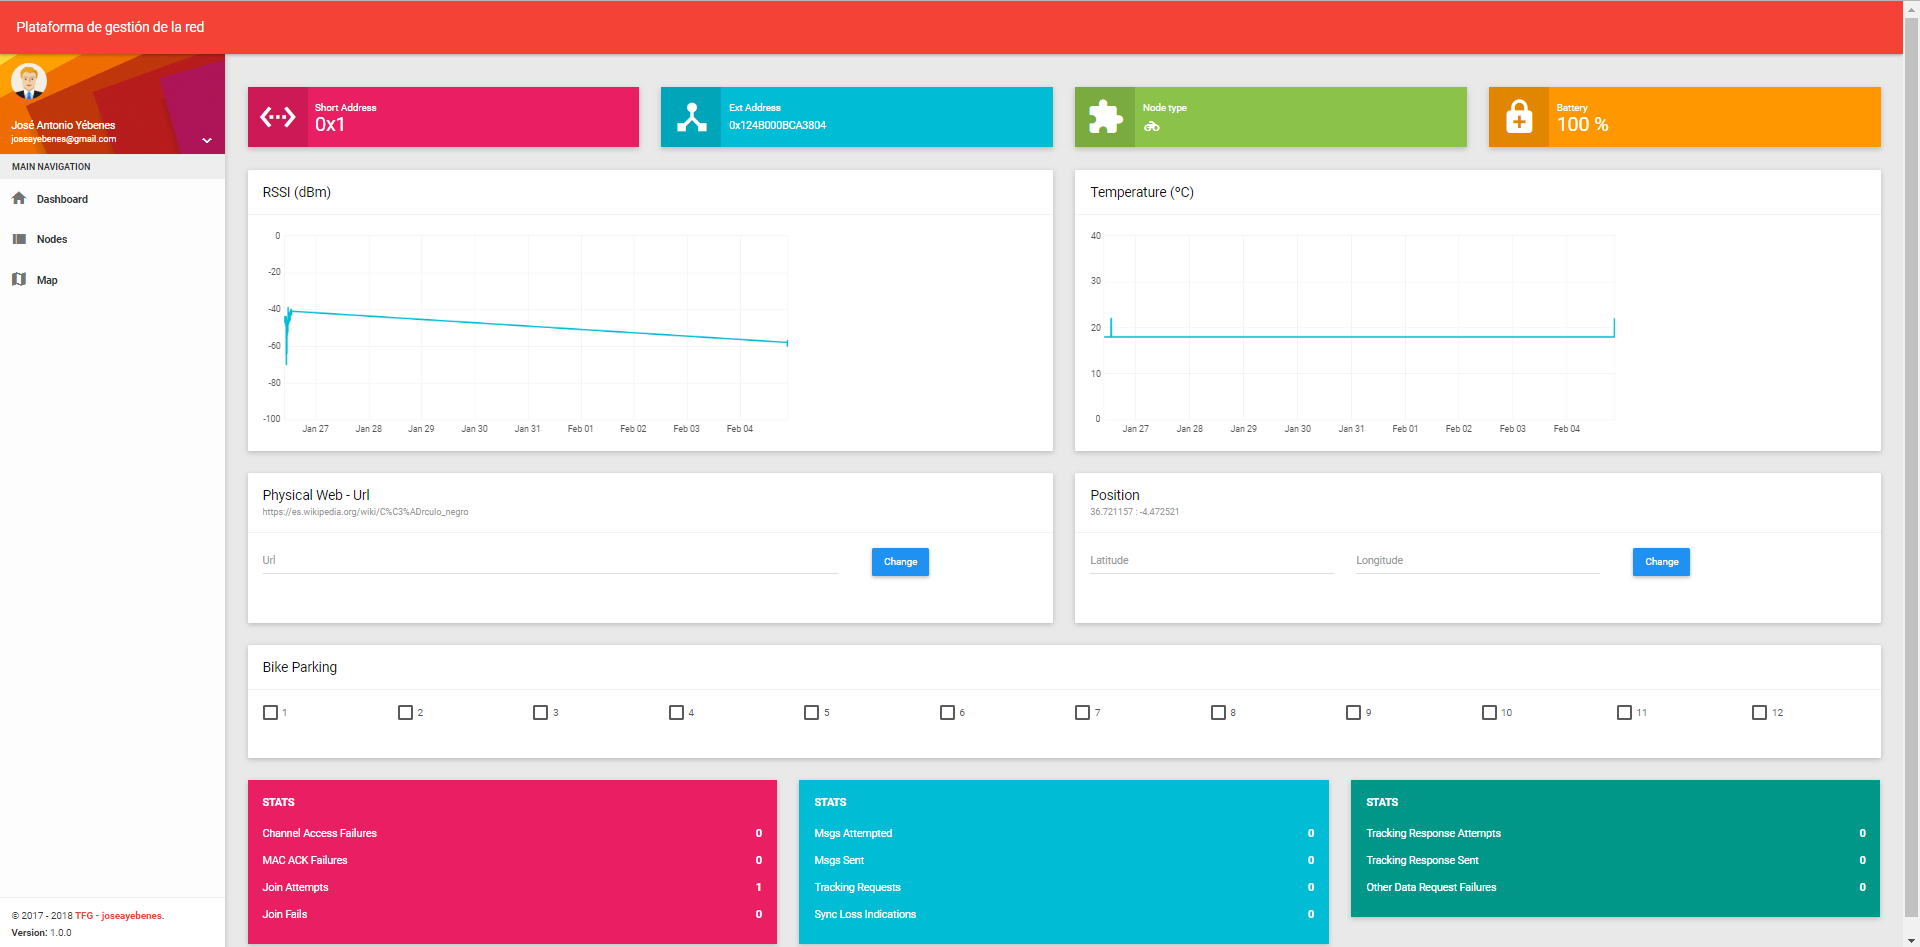
\includegraphics[width=\textwidth]{graphs/screenWebNodeBikeDetails.PNG}
	\caption{Panel de administraci�n de un tipo parking de bicicletas}
	\label{fig:screenWebNodeBikeDetails}
\end{figure}

\sectionx{Mapa}

Desde la web tambi�n es posible observar donde est� cada nodo en la red, para ello accediendo desde la barra lateral a la opci�n ``\textit{Map}'' se observa un mapa como el que se puede observar en la figura \ref{fig:screenWebMap}. En este mapa podemos observar las posiciones de los nodos que se han indicado en sus respectivos paneles de administraci�n y adem�s desde el formulario inferior es posible cambiar la posici�n del concentrador y su radio de alcance. Con esto es posible tener una idea de si alguno de los nodos se ha colocado demasiado cerca del borde del alcance del concentrador.

\begin{figure}[H]
	\centering
	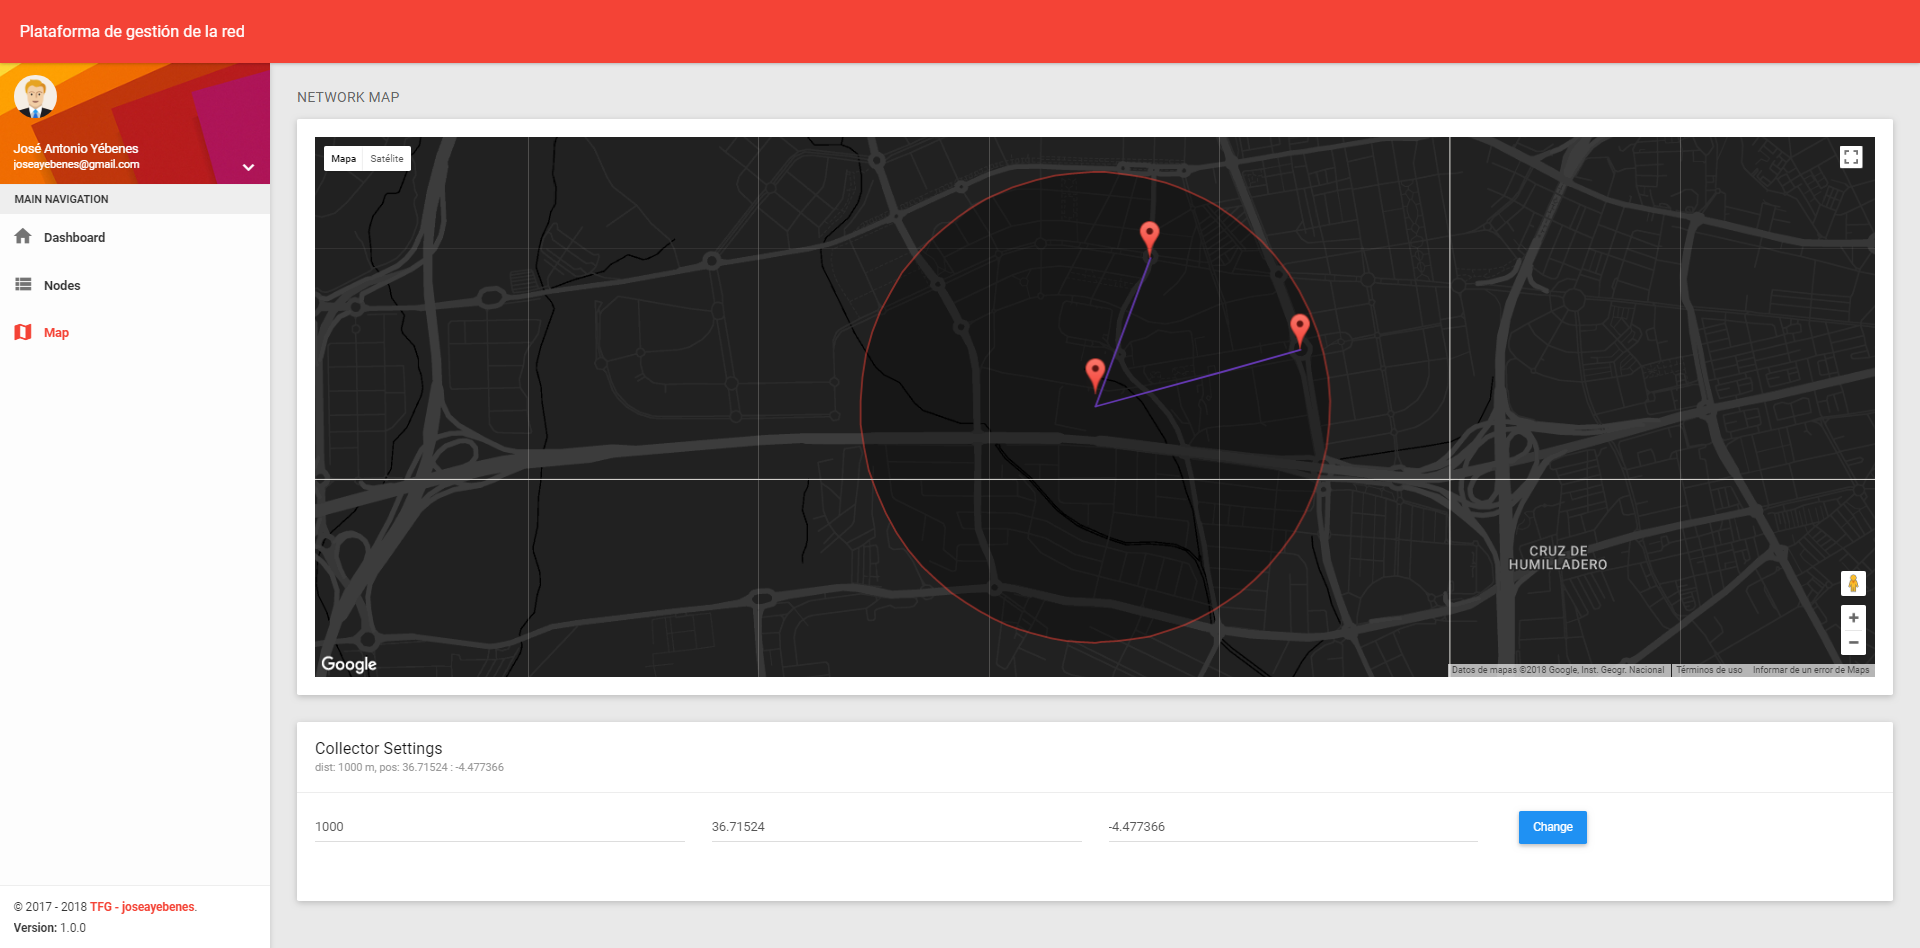
\includegraphics[width=\textwidth]{graphs/screenWebMap.PNG}
	\caption{Vista del mapa con las posiciones de los nodos}
	\label{fig:screenWebMap}
\end{figure}

\chapterend{}
%\input{D3.AppendixC.tex}

% Formato de documento en la parte final.
\backmatter
%Hace que los cap�tulos y t�tulos nivel inferior no aparezcan numerados (lo que es ideal para conclusiones o notas finales).

% Bibliograf�a
%%%%%%%%%%%%%%%%%%%%%%%%%%%%%%%%%%%%%%%%%%%%%%%%%%%%%%%%%%%%%%%%%%%
%%% Documento LaTeX 																						%%%
%%%%%%%%%%%%%%%%%%%%%%%%%%%%%%%%%%%%%%%%%%%%%%%%%%%%%%%%%%%%%%%%%%%
% T�tulo:		Bibliograf�a
% Autor:  	Ignacio Moreno Doblas
% Fecha:  	2014-02-01
% Versi�n:	0.5.0
%%%%%%%%%%%%%%%%%%%%%%%%%%%%%%%%%%%%%%%%%%%%%%%%%%%%%%%%%%%%%%%%%%%%

% Encabezamiento %
\pagestyle{fancy}
\fancyhead[LE,RO]{\thepage}
\fancyhead[LO]{Bibliograf�a}
%\fancyhead[RE]{Parte \thepart \rightmark} %
\fancyhead[RE]{\nouppercase{\rightmark}} %

%Inclusi�n de bibliograf�a%
\bibliography{E2.Bibliografia} %�sese el nombre del fichero sin extensi�n

%Inclusi�n en el �ndice (Tabla de contenidos)
\addcontentsline{toc}{chapter}{Bibliograf�a}

%Formateo de estilo de bibliograf�a
% Otros formatos: plain, unsrt, abbrv
%  plain: las entradas se ordenan alfab�ticamente y se etiquetan con un n�mero (p.ej., [1])
% unsrt: igual que plain, pero aparecen en orden de citaci�n.
% alpha: el etiquetado se hace por autor y a�o de publicaci�n (p.ej., [Knu66]).
% abbrv: igual que alpha, pero m�s abreviado.
\bibliographystyle{alpha}

%Impresi�n de todas las entradas bibliogr�ficas
\nocite{*}

\chapterend

% �ndice alfab�tico%
%%%%%%%%%%%%%%%%%%%%%%%%%%%%%%%%%%%%%%%%%%%%%%%%%%%%%%%%%%%%%%%%%%%%
%%% Documento LaTeX 																						%%%
%%%%%%%%%%%%%%%%%%%%%%%%%%%%%%%%%%%%%%%%%%%%%%%%%%%%%%%%%%%%%%%%%%%
% T�tulo:		Glosario (index)
% Autor:  	Ignacio Moreno Doblas
% Fecha:  	2014-02-01
% Versi�n:	0.5.0
%%%%%%%%%%%%%%%%%%%%%%%%%%%%%%%%%%%%%%%%%%%%%%%%%%%%%%%%%%%%%%%%%%%%

\pagestyle{fancy}
\fancyhead[LE,RO]{\thepage}
\fancyhead[LO]{�ndice Alfab�tico}
%\fancyhead[RE]{Parte \thepart \rightmark} %
\fancyhead[RE]{\nouppercase{\rightmark}} %

%index of contents
\phantomsection
\addcontentsline{toc}{chapter}{�ndice alfab�tico}
\printindex


%Example 	Index Entry 	Comment
%\index{hello} 	hello, 1 	Plain entry
%\index{hello!Peter} 	  Peter, 3 	Subentry under 'hello'
%\index{Sam@\textsl{Sam}} 	Sam, 2 	Formatted entry
%\index{Lin@\textbf{Lin}} 	Lin, 7 	Same as above
%\index{Jenny|textbf} 	Jenny, 3 	Formatted page number
%\index{Joe|textit} 	Joe, 5 	Same as above
%\index{ecole@\'ecole} 	�cole, 4 	Handling of accents
%\index{Peter|see{hello}} 	Peter, see hello 	Cross-references
%\index{Jen|seealso{Jenny}} 	Jen, see also Jenny 	Same as above

\chapterend

\end{document}